\documentclass[11pt]{article}
\usepackage{amsmath,amsfonts}
\usepackage[numbers,sort&compress]{natbib}
\usepackage{times}
\usepackage[left=2.54cm,top=2.54cm,right=2.54cm,bottom=2.54cm,bindingoffset=0.0cm]{geometry}
\usepackage{setspace}
\usepackage{enumerate}
\usepackage{enumitem}
\usepackage{wrapfig}
\setcounter{secnumdepth}{0}
\usepackage{fullpage}
\usepackage{titlesec}
\titleformat{\section}{\large\bfseries}{\thesection}{1em}{}
\titleformat{\subsection}{\bfseries}{\thesubsection}{1em}{}
\usepackage{parskip} % skip paragraph indentations
\usepackage{lipsum}
\usepackage{hyperref}
\usepackage{graphicx}
\usepackage{amssymb}
\usepackage[x11names]{xcolor}
\usepackage{hyperref}
\usepackage{enumitem}
\usepackage{booktabs}
\usepackage{amsmath}
\usepackage{amssymb}
\usepackage{mathrsfs}
\usepackage{caption} \captionsetup[table]{singlelinecheck=false} %makes table captions left-justified
\usepackage{framed} % to add frames around comments
%\hypersetup{backref,colorlinks=false,
%    urlbordercolor=LightSkyBlue4,          % color of internal links
%    citebordercolor=SpringGreen4,        % color of links to bibliography
%    filebordercolor=magenta,      % color of file links
%    linkbordercolor=Red3, pdfborderstyle={/S/U/W 1.5}}
\newcommand{\Prob}[1]{\Pr{\left( #1 \right)}}
\newcommand{\q}[1]{``#1''} % easier way to get double quotes
\newcommand{\argmin}{\text{argmin}}
\usepackage{authblk} % for title page
\renewcommand\Affilfont{\fontsize{10}{10.8}\itshape}
\renewcommand\familydefault{\sfdefault} 
\usepackage{datetime2}
%\renewcommand{\dateseparator}{-}
\usepackage{atbegshi}% http://ctan.org/pkg/atbegshi -- removes blank page at start of doc
\AtBeginDocument{\AtBeginShipoutNext{\AtBeginShipoutDiscard}}
\setcounter{page}{0}

\lhead{Learning about signals of quality can be a good strategy} 


\begin{document}
\noindent
\title{Learning about signals of quality can be better than using an innate signal assessment strategy} 
\author{}
\date{} 
\maketitle

%New target journal: Proc B 
%instructions: http://rspb.royalsocietypublishing.org/author-information
% open access: https://royalsociety.org/journals/authors/open-access/

%%%%%%%%%%%%%%%%%%%%%%%%%%%%%%%%%%%%
\linenumbers

\section*{Lay summary}
Animals that live in groups often need accurate information about their group mates and there are several strategies that animals can use to make assessments of their peers. Some animals learn to recognize each of their group mates, but others use a signal to infer something about the quality of conspecifics. We find that social assessment is always easier in small groups and when animals have long memories. We also find that learning about a signal of quality is often better than using an innate rule-of-thumb to infer quality from signal.

% % TERMS:
% individual recognition vs signal-based assessment strategies
% categorical vs rule-based strategies for inferring quality from signal

% STYLE NOTES:
% - how to treat rule / rule of thumb? EB: I'm going with rule-of-thumb but change if you prefer rule of thumb.

%%%%%%%%%%%%%%%%%%%%%%%
\section*{Abstract}
%%%%%%%%%%%%%%%%%%%%%%%
Animals in social groups benefit from having accurate information about their group mates. In many species, animals display a signal that is correlated with a property of interest, such as dominance or health. An animal can then use the signals displayed by its group mates to make inferences about their quality. Alternatively, some animals can use individual recognition to learn about each of their peers. Much is known about the the evolution of traits that are used as either signals of quality or for individual recognition, but there are few studies that address the evolution of the assessment strategies themselves. We develop and analyze a theoretical model of an animal social group, in which the animals assess each other using different strategies: three signal-based assessment strategies, as well as individual recognition. First, we find that the animals have more accurate assessments of each other when they live in larger groups and have longer memories, regardless of how the assessment strategy they use. Second, we find that signal-based assessment strategies are more likely to evolve in species that live in large groups, that have short memories, and who cannot invest a lot of time in learning. Finally, contrary to the assumption commonly made in studies of signals of quality, we find that learning about a signal is better than using an innate rule-of-thumb, except if the animals live in \emph{very} large groups and have \emph{very} short memories. These results generate testable predictions for when different assessment strategies should evolve and show that we should not always expect evolution to lead to greater cognitive complexity. 


\textbf{Keywords:} badge, cognition, evolution, learning, recognition, signal, social groups

\newpage
%%%%%%%%%%%%%%%%%%%%%%%
\section*{Introduction} 
%%%%%%%%%%%%%%%%%%%%%%%
%% SOCIAL INFORMATION
Animals in social groups benefit from having accurate information about their group mates \citep{Seyfarth:2010bh}. For example, an animal can make a better decision about whom to fight if it knows something about the dominance ~\citep{Waal:1986ys,Cowlishaw:1990vn,Bergman:2003qf,Seyfarth:2005ve,Flack:2006uq,Hobson:2015uq} or resource holding potential~\citep{Rhijn:1980uq,Freeman:1985kl,Dick:1990cr,Lemel:1993ve,Part:1997ys} of the other members of its group. Conversely, knowledge about other animals' dominance can help an animal make decision about with whom to ally itself \citep{Engh:2005qp}. A female can  make a better decision about whom to mate with if she has some information about a male's likelihood of investing in parental care~\citep{Qvarnstrom:1997fk,McGlothlin:2007au,Olsen:2010uq} or his health~\citep{Folstad:1992kx,Loyau:2005nx}. In addition to affecting how animals make decisions about social interactions, the information that animals have about each other can affect the type of social structure that emerges in their group \citep{Dugatkin:2004hz,Hobson:2015uq,Brush:2018ss}. In order to understand the evolution of sociality, it is therefore important to understand how animals make assessments of each other and how strategies for doing so have evolved.  

%% SIGNAL-BASED ASSESSMENT
One class of strategies for making social assessments is based on signals. There are many examples of species in which one trait acts as a signal of another less visible trait. When the property of interest is an animal's resource holding potential, the signal is called a badge of status \citep{dawkins1978signals,Rohwer:1981vn,Rohwer:1982fk,Ripoll:2004vn,sheehan2016evotradeoff}. A classic example of this is provided by house sparrows (\emph{Passer domesticus}), in which the size of a male's bib is correlated with his dominance \citep{Veiga:1993fk,Veiga:1995ys}. Badges of status have also been demonstrated in several other species of birds (e.g., \citep{Remy:2010fk,Olsen:2010uq,Lemel:1993ve,Tibbetts:2009kx}), mammals (e.g., \citep{Gerald:2001zm}), reptiles (e.g., \citep{Fox:1990hd}), and insects (e.g., \citep{Tibbetts:2004kx}). Signals can also provide information about other properties. For example, some species of birds have signals that communicate their current health status \citep{Folstad:1992kx,Loyau:2005nx}. In humans, a smile may be a signal of a person's likelihood of cooperating \citep{Schug:2010be}. Once such a signal has evolved, animals can use the signals displayed by their peers to make estimates of the property of interest, be it resource holding potential, health, likelihood of cooperating, or anything else.

It is difficult to determine how animals actually use a signal to assess conspecifics. In order to identify that a trait is a quality signal, scientists usually test for a statistically significant linear relationship between the putative signal and a property of interest (e.g., \citep{Rohwer:1981vn,Rohwer:1982fk,Ripoll:2004vn,Tibbetts:2004kx}). This may reflect the animals' actual strategy for using the quality signal: the animals may use the linear relationship as a rule dictating how to map signal to quality. While it is possible that an animal would be born knowing such a rule, it is also plausible that they would have to learn it over the course of interacting with conspecifics. A linear rule, however, is not the only way to infer quality from signal, even if the two are linearly related. Many cognitive processes in both humans and non-human animals are based on a categorical perception of the world \citep{Harnad:1990ux}. Both sound (e.g., \citep{Wyttenbach:1996wj,Nelson:1989rt}; reviewed in \citep{Bornstein:1987ec,Ehret:1987jh}) and color (e.g., \citep{Lim:2016ye}; reviewed in \citep{Bornstein:1987ec}) are perceived categorically by different types of animals. Animals could use a categorization strategy to make inferences about the quality of their peers based on the signals they display. For example, a house sparrow might categorize conspecifics by whether their bibs are large or small and subsequently learn that birds with large bibs have high resource holding potential and birds with small bibs have low resource holding potential.
%\textbf{(NOTE: this work isn't published yet (Steve Nowicki presented a talk at ABS this summer), maybe just have as a hypothetical example without citation??)}.   
%NOTE from EB: I changed it to house sparrow just so it didn't feel totally out of the blue that we're bringing zebra finches into the picture and I think the example still makes sense. Thanks for the name!
 
%% INDIVIDUAL RECOGNITION
In contrast to using signals to assess one's peers, an animal can simply recognize and learn about each other animal individually. Individual recognition has been demonstrated in many species and can be based on visual, olfactory, or auditory traits (reviewed in \citep{Tibbetts2007IndividualDifferent}). In order for individual recognition to work, an animal must be able to distinguish each of its peers. If an animal has only a limited ability to discriminate between its peers, it may resort to learning about categories of similar-looking animals. Individual recognition can therefore be thought of as extremely fine categorical recognition \citep{Barnard:1979fk}. Such a spectrum from coarse-grained to fine-grained perceptive abilities has actually been demonstrated within the group of paper wasps: some species distinguish between other wasps based on the number of black patches on their face, a relatively coarse trait \citep{Tibbetts:2004kx}, whereas in other species, wasps can recognize specific individuals based on their unique facial patterns \citep{Tibbetts:2002ys}. 

%% BIG UNKNOWN QUESTION
Regardless of how the assessment is being made, there are two things that have to be present in order to have a functional system of social assessment: (1) a trait that is used as either a quality signal or an identity signal and (2) an assessment strategy that is either signal-based or recognition-based.  On the signal side, much work has been done to understand when quality signals or badges of status should be expected to evolve (e.g., \citep{Whitfield:1987tg,Rohwer:1975fk,Rohwer:1982fk,Dawkins:1991ly,Johnstone:1995vn,Lachmann:1998fk,Tibbetts:2009kx}). For example, in birds, badges of status seem to evolve in species that live in large and fluid groups in the non-breeding season \citep{Tibbetts:2009kx}. There are also many studies that have identified the circumstances that facilitate the evolution of identity signals \citep{Rohwer:1975fk,Whitfield:1987tg,Sheehan:2009we,Pollard:2011te,Sheehan:2014fk}. In particular, identity signals are more likely to evolve in species that have complex social structures or highly territorial behavior \citep{Tibbetts2007IndividualDifferent}. On the assessment side, we do know some factors that should facilitate the evolution of individual recognition. For example, there needs to be sufficient variability in the trait that will be used as an identity signal \citep{Sheehan:2014fk}. Individual recognition is also more likely to evolve in species where animals can avoid costly fights by recognizing which conspecifics to avoid \citep{DEttorre:2005nu}.  \citet{sheehan2016evotradeoff} pursued a thought experiment in which they compared the errors and learning time associated with a signal-based assessment strategy and individual recognition and made predictions about when one or the other would be preferable. 
%They predicted that signal-based assessment strategies will not be affected by the number of interactions a pair of animals engages in or the size of the social group, whereas individual recognition should improve over time and become more difficult in larger groups \citep{sheehan2016evotradeoff}. 
They predicted that individual recognition would be a better strategy for animals that live in small groups and have many opportunities to learn about each other \citep{sheehan2016evotradeoff}. Quantitative support of these qualitative predictions was left for future work. Despite the fact that \citet{sheehan2016evotradeoff} identified this as an important problem, there are no theoretical models that compare the performance of a signal-based assessment strategy to that of individual recognition. 

%%MEMORY
Whether a signal-based or recognition-based assessment strategy will evolve in a particular species will depend on the animals' cognitive abilities. As we explained above, individual recognition can only work if the animals have sufficiently fine perception. Memory is an additional cognitive constraint. If animals use individual recognition, they must remember the quality of each of their peers, which can become prohibitively difficult in large groups  \citep{Rohwer:1982fk,Solberg:1997uq}. It can become even more problematic if animals have to remember the relationships between pairs of other animals ~\citep{Seyfarth2015SocialCognition}. Even humans are thought to be limited in terms of the number of people we can recognize. Previous work has hypothesized that humans can only remember the faces of about 150 people \citep{Dunbar:1993zr,Hill:2003ly}, which may have limited group size over the course of human evolution~\citep{Dunbar:1992ys,Dunbar:1993zr}. On the other hand, if animals use a linear rule to make assessments about their peers, there are essentially two parameters to remember: the slope and intercept of the line. Similarly, if animals categorize their peers, they only have to remember as many pieces of information as there are categories. These strategies therefore may be more likely to evolve in a species with poor memory.

%%UTILITY OF ASSESSMENT
Whether a signal-based or recognition-based assessment strategy will evolve in a particular species will also depend on the relative importance of making accurate assessments versus making assessments quickly. Animals use the information they have about their group mates to decide how to interact with them in the future. If their assessments of each other are inaccurate, they will make inappropriate decisions and incur costs. For example, it would be costly for an animal to steal food from a much stronger animal that he incorrectly perceived as weak. On the other hand, individuals are constrained in the total amount of effort and time that they can devote to assessing each other \citep{MacIver:2010ve}. Additionally, if interactions are aggressive, engaging in more interactions than necessary can lead to injury. There is an inherent tradeoff between accuracy and speed because waiting longer and gathering more information will tend to improve the accuracy of an animal's assessment. Animals that incur high costs from having inaccurate assessments should take the time to learn as much as they can about their peers, while animals that incur high costs from interacting should use a ``quick and dirty" strategy that allows them to gather a moderate amount of information very quickly. 

Our goal in this paper is to understand when either signal-based assessment strategies or individual recognition should be expected to evolve.  In order to do so, we developed an agent-based model of an animal social group in which animals assess each other's quality through dyadic interactions and incur costs based on these assessments. We first find that animals using any assessment strategy have more accurate opinions of their peers when they live in small groups, have long memories, and invest a lot of time in learning. Second, we find that a signal-based assessment strategy is better than individual recognition when animals live in large groups, hove short memories, and cannot invest a lot of time in learning. Finally, we find that under many circumstances learning about a signal of quality is better than using an innate rule-of-thumb. In general, our results conform to the predictions of \citet{sheehan2016evotradeoff}, although we extend their thought experiment by analyzing both innate \emph{and} learned signal-based assessment strategies (rather than just innate), and by considering a categorical assessment strategy that grades into individual recognition. 
 

%%%%%%%%%%%%%%%%%%%%%%%
\section*{Model } 
%%%%%%%%%%%%%%%%%%%%%%%

%\subsection{Interactions and quality assessment}
We consider a group of animals containing $N$ individuals (see Table~\ref{tab:vars2} for parameter descriptions). We assign each animal a quality value $q_i$ and a signal $s_i$. Quality can be thought of, for example, as fighting ability, resource holding potential, body size, body condition, or any other property about which it would be beneficial to have accurate information and which it may be difficult to estimate without interacting with an animal. The signal is an arbitrary trait that other animals can measure without interacting with a focal animal.  We assume that the signal can be used either as a quality signal or for individual recognition (although the types of traits that can be used  as quality signals or for individual recognition are likely different \citep{Dale:2001dv}).

Specifically, we draw quality values $\{q_1,\dots,q_N\}$ from a normal distribution with mean $0$ and standard deviation $\sigma_\text{q}$. We then generate $N$ signal values $\{s_i\}$ such that 
%$\min_i{s_i}\approx -1$, $\max_i{s_i}\approx 1$, and 
$\max_i\{s_i\}-\min_i\{s_i\}\approx 2$ and the sample correlation between $\{q_i\}$ and $\{s_i\}$ is precisely $\rho$. 
The higher $\rho$ is, the more informative the signal is about the underlying quality of the animals. 

We consider two classes of strategies which the animals can use to assess each other: (1) a linear rule that maps signal to quality, which can be either innate or learned, and (2) categorization, which becomes individual recognition when the animals can perceive small enough differences to be able to distinguish among all of their peers. For each assessment strategy, the animals interact and assess each other for $T$ timesteps. At each point in time, two animals, $i$ and $j$, are chosen randomly to interact. Through this interaction, each receive noisy information about the other's quality: $i$ experiences a quality value of $\hat{q}_j=q_j+\xi$, where $\xi$ is drawn from a normal distribution with mean $0$ and standard deviation $\sigma_\xi$, and vice versa for $j$. 

After this interaction, every animal in the group updates its assessment of every other animal, as described below. For each assessment strategy, $a_{ij}(t)$ is animal $i$'s assessment of $j$'s quality at timestep $t$. Note that we do not allow for observational learning, even though it is known to be important in many systems (e.g., \citep{Freeman:1985kl,Holekamp:1991nx,Schaik:2011oq,Hobson:2015uq,Seyfarth2015SocialCognition}). The main effect of observational learning would be to increase the rate at which the animals can learn about each other, but it would not qualitatively affect our results. 


\subsection*{Linear rule}
We first describe animals that use a linear rule to infer quality from signal. In this case, each animal's assessment is given by
\begin{linenomath*}
\begin{equation*}
a_{ij}(t)=m_i(t)s_j+b_i(t),
\end{equation*}
\end{linenomath*}
where $m_i(t)$ and $b_i(t)$ are the slope and intercept that $i$ believes describe the linear relationship between signal and quality at timestep $t$. In words, when animal $i$ observes that animal $j$ displays signal $s_j$, animal $i$ infers that $j$ has quality $m_i(t)s_j+b_i(t)$. When the rule is innate, there are values $m$ and $b$ such that $m_i(t)=m$ and $b_i(t)=b$ for each individual $i$ and timestep $t$. In words, the slope and intercept of the linear rule are the same for all members of the group and do not change over time. Animals can use this rule immediately and do not need to spend any time learning.  An innate rule has presumably evolved over time to describe the average relationship between signal and quality. To model this, we generate $10,000$ groups with quality and signal values as described above. In each group $g$, we find the slope $m_{g}$ and intercept $b_{g}$ of the best-fitting line through the points given by $\{s_i\}$ on the x-axis and $\{q_i\}$ on the y-axis. We then take the average of these over all $10,000$ groups, so that $m=\sum_{g} m_{g}/10000$ and $b=\sum_{g}b_{g}/10000$. 

%\subsection*{Learned rule}
We also allow animals to learn a rule to assess each other's quality. In this case, all members of the group are initially naive: at $t=0$, no animal has an opinion of any other or any estimate of the slope and intercept of the signal-quality relationship. The animals have a ``memory window" $w$ such that each animal remembers any interactions that have occurred within the last $w$ timesteps. From each of these recent interactions, an animal $i$ stores the signal of its partner, $s_j$, as well as noisy information about its quality, $\hat{q}_j$.  Then $m_i(t)$ and $b_i(t)$ are the slope and intercept from the best-fitting line through the points given by the observed $\{s_j\}$ on the x-axis and the observed $\{\hat{q}_j\}$ on the y-axis.   

\subsection*{Categorization}
We next describe animals that perceive their conspecifics' signals categorically. In this case, the way animals categorize their peers depends on the magnitude of the differences in signals they can perceive. Specifically, an animal can only distinguish between two other animals $j$ and $k$ if $|s_j-s_k|>\delta$, that is, if their signals are sufficiently different. If the animals have coarse perceptive abilities, the parameter $\delta$ will be large, and if the animals have fine perceptive abilities, the parameter $\delta$ will be small. When $\delta=0$, the animals can discriminate among every individual in their group, so categorization becomes individual recognition. We consider a representative set of values for $\delta$, specifically $0$, $0.25$, $0.5$, $0.75$, and $1$.

Before any interactions take place, each animal in the group divides its peers into categories. It does so by picking another animal, $j$, at random. All animals whose signals are within $\delta/2$ of $s_j$ are put in the same category. Then the focal animal picks an uncategorized animal at random, $k$, forming a second category of all uncategorized animals whose signals are within $\delta/2$ of $s_k$. The process continues until every animal in the group has been assigned a category. The parameter $\delta$ can therefore be thought of as ``category width."  Different animals will categorize the group differently and may perceive different numbers of categories. Figure \ref{category_diagram} shows one example of this process for various values of $\delta$. When $\delta=0$, there are as many ``categories" as there are animals. As category width increases, animals will use fewer categories, each of which will contain more animals  (Figure \ref{category_diagram}). 

%\subsection*{Updating assessments}
As with the learned rule above, at first, the group consists entirely of naive animals. Again, each animal has a memory window $w$ such that it remembers categories it has encountered in the last $w$ timesteps and forgets its opinion of categories it has not interacted with within the last $w$ timesteps. When two animals engage in an interaction, each animal updates its assessment of the other to be the weighted average of its old estimate and the new information it has received. Specifically, if $i$ already has an estimate of $j$'s category, its new assessment of the category will be
\begin{linenomath*}
\begin{equation*}
a_{ij}(t+1)=(1-r)a_{ij}(t)+r\hat{q}_j,
\end{equation*}
\end{linenomath*}
where $\hat{q}_j$ is the noisy information received about $j$'s quality and $r$ is the ``updating rate" describing how much each animal changes its assessment based on the interaction. As with $\delta$, we choose a representative set of values of $r$ to explore, specifically, $0.05$, $0.1$, $0.25$, and $0.5$. Animal $i$ simultaneously updates its opinions of all the other animals in the same category as $j$.
If $i$ has not previously interacted with animals in $j$'s category or if $i$ has forgotten about the category, its new estimate of the category is
\begin{linenomath*}
\begin{equation*}
a_{ij}(t+1)=r\hat{q}_j.
\end{equation*}
\end{linenomath*}
%In words, an animal's baseline opinion of a stranger is $0$, the average quality value of any group. 

According to \citet{sheehan2016evotradeoff}, what distinguishes an assessment strategy that relies on quality signals from individual recognition is that, with a quality signal, an animal can know something about a conspecific based solely on the signal it displays without having had to interact with it. In our model, this is true for animals using categorization with category width $\delta>0$, as well as for animals using either an innate or learned rule. In other words, both the categorization and rule strategies we analyze can be considered signal-based assessment strategies that differ in whether they are innate or learned and in how animals infer quality from signal (Figure \ref{schematic}). 
 
\subsection{Assessment errors }
For each assessment strategy and each combination of parameters, we simulate $25$ groups undergoing the processes just described.  To quantify how well the animals assess each other, we measure how accurately and how quickly they assess each other's quality. The error of animal $i$'s assessment of animal $j$ at time $t$ is $e_{ij}(t)=|a_{ij}(t)-q_j|$. For a given combination of parameters, we take the average error that any animal makes in its assessments of the rest of its group over all groups, 
\begin{linenomath*}
\begin{equation*}
\epsilon(t) = \frac{\sum_{\text{groups}}\sum_i\sum_{j\in \mathscr{O}_i(t)}e_{ij}(t)}{25N|\mathscr{O}_i(t)|},
\end{equation*}
\end{linenomath*}
where $\mathscr{O}_i(t)$ is the set of animals about whom $i$ has an opinion at time $t$.

In Figure \ref{tradeoff} we show representative examples of how the average error of animals using each assessment strategy changes over time.  For animals using either a learned rule or categorization, as the animals learn about each other, $\epsilon(t)$ decreases until it reaches an equilibrium value (Figure \ref{tradeoff}). At first, animals are more or less guessing about the quality of their peers, which results in a high average error. When learning is difficult, for example because the animals' memory is poor or there are many animals to learn about, the average error barely decreases from its initially high level (Figure \ref{tradeoff}). When learning is easier, for example because the animals can remember more interactions, because there are fewer animals to learn about, or because the signal is very informative, average error decreases dramatically over time and can even approach $0$ (Figure \ref{tradeoff}).  

\subsection{Assessment costs }
We are interested in identifying which assessment strategy is least costly, as this is the strategy we would expect to evolve. To do so, we must measure the cost associated with each assessment strategy. Animals incur costs when they have inaccurate estimates of their peers' quality and by continuing to spend time learning about each other when they could be engaging in other activities. We thus quantify the cost incurred at time $t$ as 
\begin{linenomath*}
\begin{equation*}
C(t) = 2c\epsilon(t) +(1-c)\frac{t}{T}.
\end{equation*}  
\end{linenomath*}
In words, the total cost $C$ is a weighted average of error and the time spent learning. The parameter $c$ ranges from $0$ to $1$ and quantifies the tradeoff between accuracy and speed: when $c$ is close to $1$, errors are very costly but the time spent learning is not very costly, whereas when $c$ is close to $0$, the time spent learning is very costly but errors are not very costly. The factors of $2$ and $1/T$ ensure that the two costs are on the same scale, namely between $0$ and $1$. 
The cost function $C(t)$ initially decreases, reaches a minimum, and either stays constant at that value or starts to increase as the animals engage in more interactions (Figure \ref{tau}). 

As we will show, increasing an animal's memory window $w$ always improves how accurately it can learn. In reality, it may be costly for animals to invest in a longer memory. However, rather than using an arbitrary function to describe the costs of memory, we treat memory window as a fixed cognitive factor that affects how well the animals can learn and what learning strategies they should use. The interesting question of how memory itself would evolve is left for future work. Similarly, while group size $N$ and signal-quality correlation $\rho$ may evolve over time, we assume that they are fixed on the timescales we consider. 


\subsection{Optimization }
We are interested in understanding when different assessment strategies might evolve. There are variables \emph{within} each assessment strategy that could evolve over time. It seems reasonable that, if a population is using a given assessment strategy, traits affecting that strategy would evolve and reach optimal values more before an entirely novel assessment strategy could arise and reach fixation. Therefore, we first look at how to optimize the performance of a particular strategy and \emph{then} compare the performance of the optimized assessment strategies to understand when which strategy would evolve. We next describe how we optimize the performance of each assessment strategy: the learned rule, the innate rule, and categorization, which can turn into individual recognition with a category width of $\delta=0$.

One strategy that animals using any assessment strategy can vary is how many interactions they engage in before they stop learning. As we described above, eventually the cost function $C(t)$ reaches a minimum value and either plateaus or starts to increase (Figure \ref{tau}). The animals should stop gathering new information at this point because they will only incur greater costs by continuing to spend time interacting with their peers. We refer to the number of interactions at which this occurs as the stopping time $\tau$. In other words, $C(\tau)$ is the minimum cost that can be incurred for a given set of parameters. When $c$ is close to $1$, the animals will keep learning in order to improve their accuracy and $\tau$ will be high, whereas when $c$ is close to $0$, taking time to learn is costly and $\tau$ will be low. For animals using an innate rule, $\tau$ is always equal to $1$ because they do not engage in learning and cannot improve their assessments by engaging in more interactions. 

Within a population of animals using categorization, the traits of category width $\delta$ and updating rate $r$ can also evolve. For given values of the signal-quality correlation $\rho$,  group size $N$, memory window $w$, and cost of errors $c$, and for every combination of $\delta$ and $r$, we find the stopping time $\tau$ and the minimum possible cost $C(\tau)$. This allows us to find the combination of $\delta$ and $r$ that minimizes $C(\tau)$. These are the traits that we would expect to evolve in a population using categorization as its assessment strategy. In particular, if $\delta=0$ is the optimal trait, then individual recognition would be expected to evolve, whereas if the optimal value of $\delta$ is greater than $0$, then categorization would be expected to evolve.  

To compare all assessment strategies for a given signal-quality correlation $\rho$, group size $N$, memory window $w$, and cost of errors $c$, we compare the total cost of learning for animals using an innate rule, animals using a learned rule, and animals using categorization with optimized $\delta$ and $r$. We expect that the assessment strategy with the lowest cost would be able to invade a population using any other strategy.


The entire model was written in R and all model code will be released on publication on Github.

%%%%%%%%%%%%%%%%%%%%
\section*{Results}
%%%%%%%%%%%%%%%%%%%%

\subsection*{The effects of the signal-quality correlation, group size, and cognitive abilities on learning}
We first analyze how stopping time $\tau$  and average error $\epsilon(\tau)$ depend on various parameters describing the animals' learning strategies, group demographics, and cognitive abilities. Recall that stopping time $\tau$ is the number of interactions at which the animals' overall cost $C(t)$ stops decreasing and $\epsilon(\tau)$ is the average error of the animals' assessments at that point in time. Additionally, when time is not at all costly ($c=1$), the overall cost is equal to twice the animals' average error ($C(\tau)=2\epsilon(\tau)$). Category width $\delta$ and updating rate $r$ only affect stopping time and average error in animals using categorization and categorization becomes recognition when category width $\delta=0$.

For animals using categorization, category width $\delta$ and updating rate $r$ have similar effects on stopping time and average error. With higher updating rates and larger category widths, the animals gather information more quickly, but that information is noisier, either because more weight is given to the animals' noisy observations or because more animals are lumped together into the same category. Therefore, as either updating rate or category width is increased, the average error of the animals' assessments plateaus more quickly and stopping time decreases (Figure \ref{tradeoff}). When the animals have long memories, this is associated with an increase in the equilibrium level of error (Figure \ref{tradeoff}A and C). However, when the animals have short memories, this decrease in learning time is additionally associated with a \emph{decrease} in the equilibrium level of error (Figure \ref{tradeoff}B and D). In other words, when the animals have short memories, it is beneficial to gather as much information as quickly as possible, even if that information is noisier. This shows that using categorization ($\delta>0$) can be preferable to using recognition ($\delta=0$) under some circumstances. (The interactions between memory window, category width, and updating rate are shown in full in Figure \ref{interactions}.)

The signal-quality correlation $\rho$ only affects animals using signal-based assessment strategies, i.e. either type of rule or categorization with $\delta>0$, but not recognition. Signal-quality correlation does not have a strong effect on how long it takes to assess one's group mates (Figure \ref{parameters}A), but increasing the correlation dramatically reduces the errors made by animals using signal-based assessment strategies (the blue and purple curves in Figure \ref{parameters}E).

As group size $N$ increases, it takes animals longer to learn about their peers (Figure \ref{parameters}B). (Remember that animals using an innate rule do not learn and their stopping time is always equal to $1$.) As group size increases, animals using categorization or recognition make greater errors (red and purple curves in Figure \ref{parameters}F), but the error of animals using either type of rule is not strongly affected (the blue curves in Figure \ref{parameters}F).

Similarly, the animals' memory window $w$ only really affects animals using categorization and recognition. For these animals, as memory window increases, it takes longer for their assessment error to reach a plateau, so stopping time increases (red and purple curves in Figure \ref{parameters}C), but because they can remember more information, their errors are reduced (red and purple curves in Figure \ref{parameters}G). As accuracy becomes more important and the cost of errors $c$ increases, animals using any learned strategy invest more time in learning (Figure \ref{parameters}D), which helps them reduce their errors (Figure \ref{parameters}H). In summary, the effects of  signal-quality correlation, group size, memory window, and cost of errors on learning speed and learning accuracy are generally intuitive and confirm that our model is a reasonable description of some of the basic properties of a real social system. 
  
\subsection*{Optimal learning strategies for animals using categorization}
As described above, for each signal-quality correlation $\rho$, group size $N$, memory window $w$, and cost of errors $c$, we find the optimal category width $\delta$ and updating rate $r$ for animals using categorization. Remember that using $\delta=0$ means the animals are actually using individual recognition. For the optimal $delta$ to be greater than $0$, i.e. for categorization to be better than individual recognition, the signal needs to be almost perfectly correlated with quality ($\rho=0.99$) (there are only purple squares in the bottom row of Figure \ref{opt_delta}). Of the cases when $\rho=0.99$, categorization is better than recognition when the animals live in large groups (large $N$), when they have short memories (small $w$) and when it is  costly to spend time learning (small $c$) (the purple regions of Figure \ref{opt_delta}). Under these circumstances, using a category width greater than $0$ helps the animals learn more quickly and to generalize their observations to a large number of unknown animals. Conversely, animals should invest in individual recognition when the signal-quality correlation is lower or when the animals live in smaller groups, when they have long memories, and when errors are costly (the red regions of Figure \ref{opt_delta}). Note that a category width greater than $0.25$ is never optimal (Figure \ref{category_diagram}). 

For those parameters where categorization ($\delta=0.25$) is optimal, it is also optimal to use a high updating rate (Figure \ref{l}). In fact, the optimal updating rate behaves similarly to the optimal category width: a high updating rate is best when the animals live in larger groups, when they have short memory windows, and when errors are not very costly, and  (Figure \ref{l}). When animals using categorization use optimal stopping time (Figure \ref{time}), category width (Figure \ref{opt_delta}), and updating rate (Figure \ref{l}), the error with which animals assess their peers decreases as group size decreases, as memory window increases, and as the cost of errors increases (Figure \ref{error}). The optimal stopping time $\tau$ for animals using the learned rule and the resulting average error $\epsilon(\tau)$ are shown in Figures \ref{time_rule} and \ref{error_rule} respectively.


\subsection*{Optimal assessment strategy}
We now compare the overall costs of using each assessment strategy, where we assume that the animals using any strategy that involves learning are using the optimal stopping time $\tau$ and that animals using categorization are using the optimal category width $\delta$ and updating rate $r$. When we compare all the assessment strategies, we find that either a learned or innate rule is the best assessment strategy when the animals live in large groups (large $N$), when they have short memories (small $w$), and when it is costly to spend time learning (small $c$) (the blue regions of Figure \ref{best}). Conversely, individual recognition is the best strategy when the animals live in smaller groups, when they have long memories, and when errors are costly (the red regions of Figure \ref{best}). Of the parameters where a rule is preferable, an learned rule is preferable to an innate rule unless the group size is very large ($N=100$) and the memory window is very short ($w\leq500$) (intermediate blue regions of Figure \ref{best}). There are large regions of parameter space where all three assessment strategies---the learned rule, the innate rule, and individual recognition---perform almost equally (the grey regions in Figure \ref{best}). Note that there are no parameters where categorization ($\delta>0$) is the best strategy of all (Figure \ref{best}).  

%%%%%%%%%%%%%%%%%
\section*{Discussion}
%%%%%%%%%%%%%%%%%
%HERE HERE HERE

% Study question, restated/reframed
In animal social groups, having an accurate opinion about the quality of one's group mates is important in many contexts. One way that animals share information about their own quality is through a signal. There have been many studies about the evolution of quality signals, but the evolution of the strategies animals use to make inferences from those signals is less well studied. We modeled quality assessment in social groups, with animals using either a signal, which allows them to infer the quality of an unknown animal, or individual recognition, which allows them to learn about each particular individual. We considered three signal-based assessment strategies: an innate linear rule mapping signal to quality, a learned rule, and categorization of signals. Our goal was to better understand the costs and benefits of each strategy and the conditions under which each strategy might be favored. 


\subsection*{The effect of group size and cognition on learning} 
We first evaluated how various demographics and cognitive traits affect the efficacy of each strategy in isolation. We  find that agents using a signal-based assessment strategy learn more quickly and accurately when there is a strong correlation between the signal and quality. We also find that for animals that use a learned assessment strategy (a learned rule, categorization, or recognition), living in a large group or having a short memory make it more difficult to make accurate assessments. Of these strategies, recognition is the most severely affected by both group size and memory.  

Our model was inspired by the thought experiments carried out by \citet{sheehan2016evotradeoff}. They compared recognition with an innate signal-based assessment strategy, which would be most similar to the innate rule we consider. \citet{sheehan2016evotradeoff} made four qualitative predictions to which we can compare our quantitative results. First, they predicted that animals using recognition would increase their accuracy over the course of interacting with their peers and that the accuracy of an animal using an innate signal-based assessment strategy would not change over time (their Figure 1b). This agrees with our findings (our Figure \ref{tradeoff}).  Second, they predicted that the an animal using recognition would make more accurate assessments in smaller groups, but that the accuracy of an animal using an innate signal-based assessment strategy would be unaffected by group size (their Figure 1c). This also agrees with our findings (our Figure \ref{parameters}F). \citet{sheehan2016evotradeoff} considered costs that the animals incur from spending time learning about each other, as well as from investing in cognitive capacity. A third prediction they made was that the costs of assessment should increase as a function of group size for animals using individual recognition, but should be unaffected by group size for animals using an innate signal-based assessment strategy (their Figure 1d). This agrees with our findings about the time spent learning (our Figure \ref{parameters}B). Fourth, they wrote that there are ``conditions under which the reliability of quality signals and social recognition are expected to be similar" \citep{sheehan2016evotradeoff}. We find large areas of parameter space in which individual recognition, a learned rule, and an innate rule performed essentially equivalently (our Figure \ref{best}). We agree with their conclusion that the evolution of an assessment strategy in these circumstances will likely be highly contingent on history and accidents \citep{sheehan2016evotradeoff}. \citet{sheehan2016evotradeoff} made additional predictions about the effects of having traits that can change over time, as well as group dynamics that allow the group composition to change over time. These interesting factors are left for future work.

In general, our findings about an innate signal-based assessment strategy and individual recognition agree with the predictions that \citet{sheehan2016evotradeoff} made. However, in addition to considering an innate signal-based assessment strategy, we considered two learned signal-based assessment strategies: the learned rule and categorization. These strategies often behaved quite differently from the innate rule. For example, both learned signal-based assessment strategies are affected by group size, whereas the innate rule is not. Our model serves as proof of concept that learned signal-based assessment strategies can be effective and shows that specifying how exactly animals use a signal to make assessments is important.

\subsection*{Evolution of signal-based assessment strategies }

When we restrict our attention to the categorization-recognition spectrum, we find that animals using categorization incur fewer costs than those using individual recognition when the animals live in large groups, when they have short memories, and when it is costly to spend time learning. Similarly, when we compare all assessment strategies, the rule strategies are best when the animals live in large groups, when they have short memories, and when the time spent learning is costly; the innate rule is only better than the learned rule when animals live in \emph{very} large groups and have \emph{very} short memories. Conversely, individual recognition is a better strategy when the signal and quality are less highly correlated, when the animals live in small groups, when they have long memories, and when accuracy is important. 

There are circumstances under which categorization is better than individual recognition. In those cases, if categorization arises through either a genetic mutation or a learned innovation, it would likely invade and reach fixation in a population of animals using individual recognition. If a rule strategy were to arise later, it would likely invade a population of animals using categorization, but categorization could persist for some time. The rate at which new strategies arise and the order in which different strategies appear will jointly determine the evolutionary dynamics of the various assessment strategies. An analysis of these full dynamics is left for future work. 

Our findings---that signal-based assessment strategies are preferable when the animals live in large groups and when it is important to learn quickly---agrees with the predictions made by \citet{sheehan2016evotradeoff}. They also agree with previous studies that found that individual recognition is most useful in small groups \citep{Veiga:1993fk} and that badges are more likely to evolve in large groups with fluid social systems \citep{Rohwer:1975fk,Tibbetts:2009kx}. There is one major difference between our results and empirical observations: We found that signal-based assessment strategies are only valuable when the signal is very highly correlated with quality ($\rho\geq 0.9$), which is higher than the correlations that have estimated in species that use badges of status (e.g., paper wasps \citep{Tibbetts:2004kx}, house sparrows \citep{Veiga:1993fk}, swamp sparrows \citep{Olsen:2010uq}, see Table \ref{corr_examples}). One explanation for this difference is that the effect group sizes in these species is much larger than those that we consider, which would make it more likely for even a weakly informative signal to be worthwhile. Further work is needed to fully test these predictions with empirical data.

What is novel about our model is that we consider signal-based assessment strategies under which the animals have to learn about their group mates' signals, namely the learned rule and categorization. It is often assumed, without much empirical justification, that, if animals are using a quality signal to assess conspecifics, they are born with the understanding of how to do so. Our results show that not only can learning about a quality signal allow an animal to accurately and quickly assess its peers, but that the learned rule is actually the best assessment strategy under many circumstances. This suggests that we should be more circumspect in making assumptions about animals using an innate signal assessment strategy and that careful empirical work is needed to identify the strategies that animals are actually using.

In our model, we assume that there is a continuously distributed signal that is lumped into categories based on the perceptive abilities of the receivers of the signal. Instead of a continuously distributed signal, there are systems in which subsets of animals with similar quality values exhibit the same signal, so only a discrete set of signals is available to the receivers \citep{Johnstone:1994uq}. Theoretical models show that using a discrete set of signals, rather than a continuous distribution, can stabilize a signaling system. In some models, when receivers of the signal are error prone, the equilibrium set  signaling strategie only includes a finite number of signals \citep{Grafen:1993kx,Johnstone:1994uq}. In a model that allows for multiple qualities to be communicated via multiple signals, it is also the case that animals with different quality values could display the same signals \citep{Johnstone:1995vn}. In another model, allowing for such ``pooled" signals increases the likelihood of finding a signaling equilibrium \citep{Lachmann:1998fk}. We find that perceiving a discrete set of categories can make it easier for a receiver to learn about the signals, which is further evidence that discrete signals are likely to be advantageous in many natural systems.

Category width is related to the animals' perception ability: if they cannot perceive fine differences, they will be forced to categorize the signals of their group mates. Similarly, an animal may be forced to use a linear rule-of-thumb if it cannot remember or distinguish all of its peers. Our finding that both categorization and a linear rule can sometimes perform better than individual recognition is therefore somewhat counterintuitive, as one might expect that it would always be advantageous to improve one's perceptive abilities. One explanation for why animals have imperfect cognition is that there are costs involved in improving their cognition \citep{Dunbar:1992ys,Laughlin:1998ly,Laughlin:2001qf,Gavrilets:2006fk,MacIver:2010ve}. However, our results suggest that imperfect cognition itself may be adaptive. This may explain empirical examples of imperfect cognition (e.g., \citep{Kikuchi:2010ys}). Other studies have also found that the most advanced cognitive strategies are not always optimal \citep{Stephens:1991fk,Kerr:2003vn,Dunlap:2009vn}. Our work therefore contributes to our growing understanding of the circumstances that do not lead to the evolution of sophisticated cognition. 

\subsection*{Future work and conclusion}
 
By studying an abstract model of social assessment, we were able to identify the conditions under which different assessment strategies are most effective and to determine the conditions that would lead to the evolution of different strategies. There are further steps towards improving the realism of the model that will also improve our predictions about the evolution of the assessment strategies. For example, in our model, group composition never changes. However, the membership of real animal groups changes over time as animals are born, die, and move between groups. Group dynamics are expected to affect the evolution of both badges of status \citep{Rohwer:1975fk,Tibbetts:2009kx} and individual recognition \citep{Whitfield:1987tg,Veiga:1993fk}. In follow-up work, we plan to incorporate group dynamics in order to explicitly test these ideas. The other major simplifying assumption we made is that the signal does not change over time, either within an animal's lifetime or on an evolutionary timescale. Whether animals use a learned or innate strategy for inferring quality from signal can in turn affect the evolution of the signal itself \citep{Kamo:2002vi}. A complete understanding of the evolution of social assessment will require considering the full feedback loop, that is, including both the effect of the signal on the evolution of the assessment strategy and the effect of the assessment strategy on the evolution of the signal.

Learning about one's group mates is a challenge facing every animal that lives in a social group. There is a spectrum of solutions to this problem determined by the number of parameters the animals have to use: at one end, animals can use a simple linear rule to infer quality from signal or coarsely categorize conspecifics into two groups, while at the other, they can recognize every one of their peers individually.
Different conditions favor different solutions. By considering and comparing a range of solutions to the same biological problem, we have rigorously verified the intuition we and others have had about these systems. By explicitly comparing different assessment strategies, we have generated testable predictions about the types of species and social groups in which we expect one or the other to evolve. Our approach also provides intriguing insight into the social factors that shape animal cognition and the evolution of cognitive complexity. 
%%%%%%%%%%%%%%%%%%%%%%%%%%%%%%%%%%%%%%%%%%
\newpage
\bibliography{BIB_badgeVSrecog}
\bibliographystyle{jeb}

\newpage

\begin{figure}[ht]
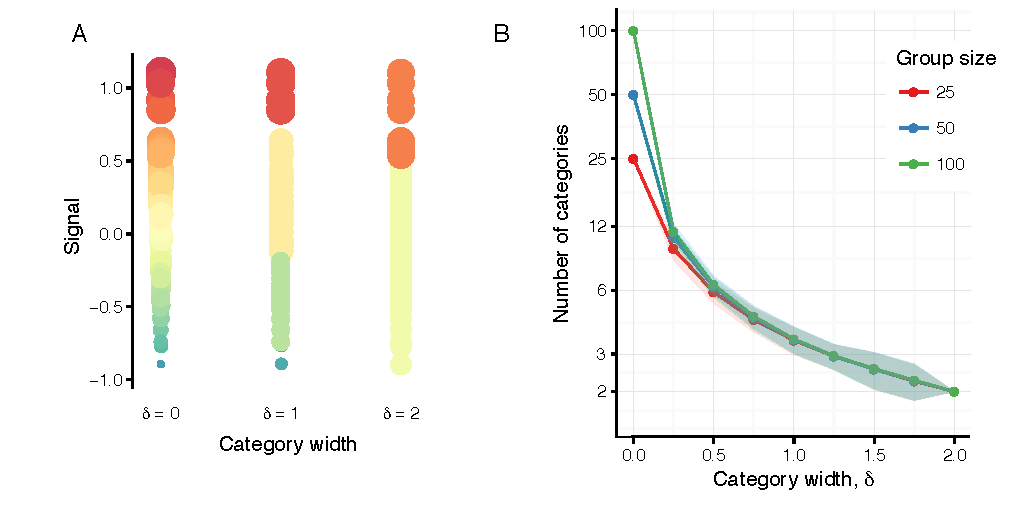
\includegraphics[width=6.85in]{figures/category_diagram.pdf}
\caption{\sffamily\small\textbf{As category width increases, the animals use fewer categories, each of which includes more animals.} 
In A we show how a given set of signals could be categorized using three different values of category widths $\delta$. The three vertical lines of dots represent the same group, with the same set of signals $\{s_i\}$. Each dot represents an animal in the group and the vertical position of a dot represents the animal's signal. In each column, animals in the same category are represented by circles of the same size and color, indicated the average signal for animals in that category. The range of signals in a given category can be no more than $\delta$. In the left column, $\delta=0$ and there are $N=100$ categories. In the middle column, $\delta=1$ and there are four categories. In the right column, $\delta=2$ and there are two categories.  In B, we show how the number of categories an animal uses depends on the category width. For a given group size $N$ and category width $\delta$, we generated $5,000$ groups with signal values $\{s_i\}$ and categorized the group according to the procedure shown in A.  Category width is on the x-axis. The average number of categories across the $5,000$ groups is on the y-axis, which is on a logarithmic scale, with the color indicating group size. The shaded areas show this average plus or minus the standard deviation across the $5,000$ groups. When $\delta=0$ there are as many categories as there are animals in the group. When $\delta=2$, it is theoretically possible for all animals to be put into the same category, but this was never observed, and instead the animals were always put into $2$ categories. }
 \label{category_diagram}
\end{figure}

\begin{figure}
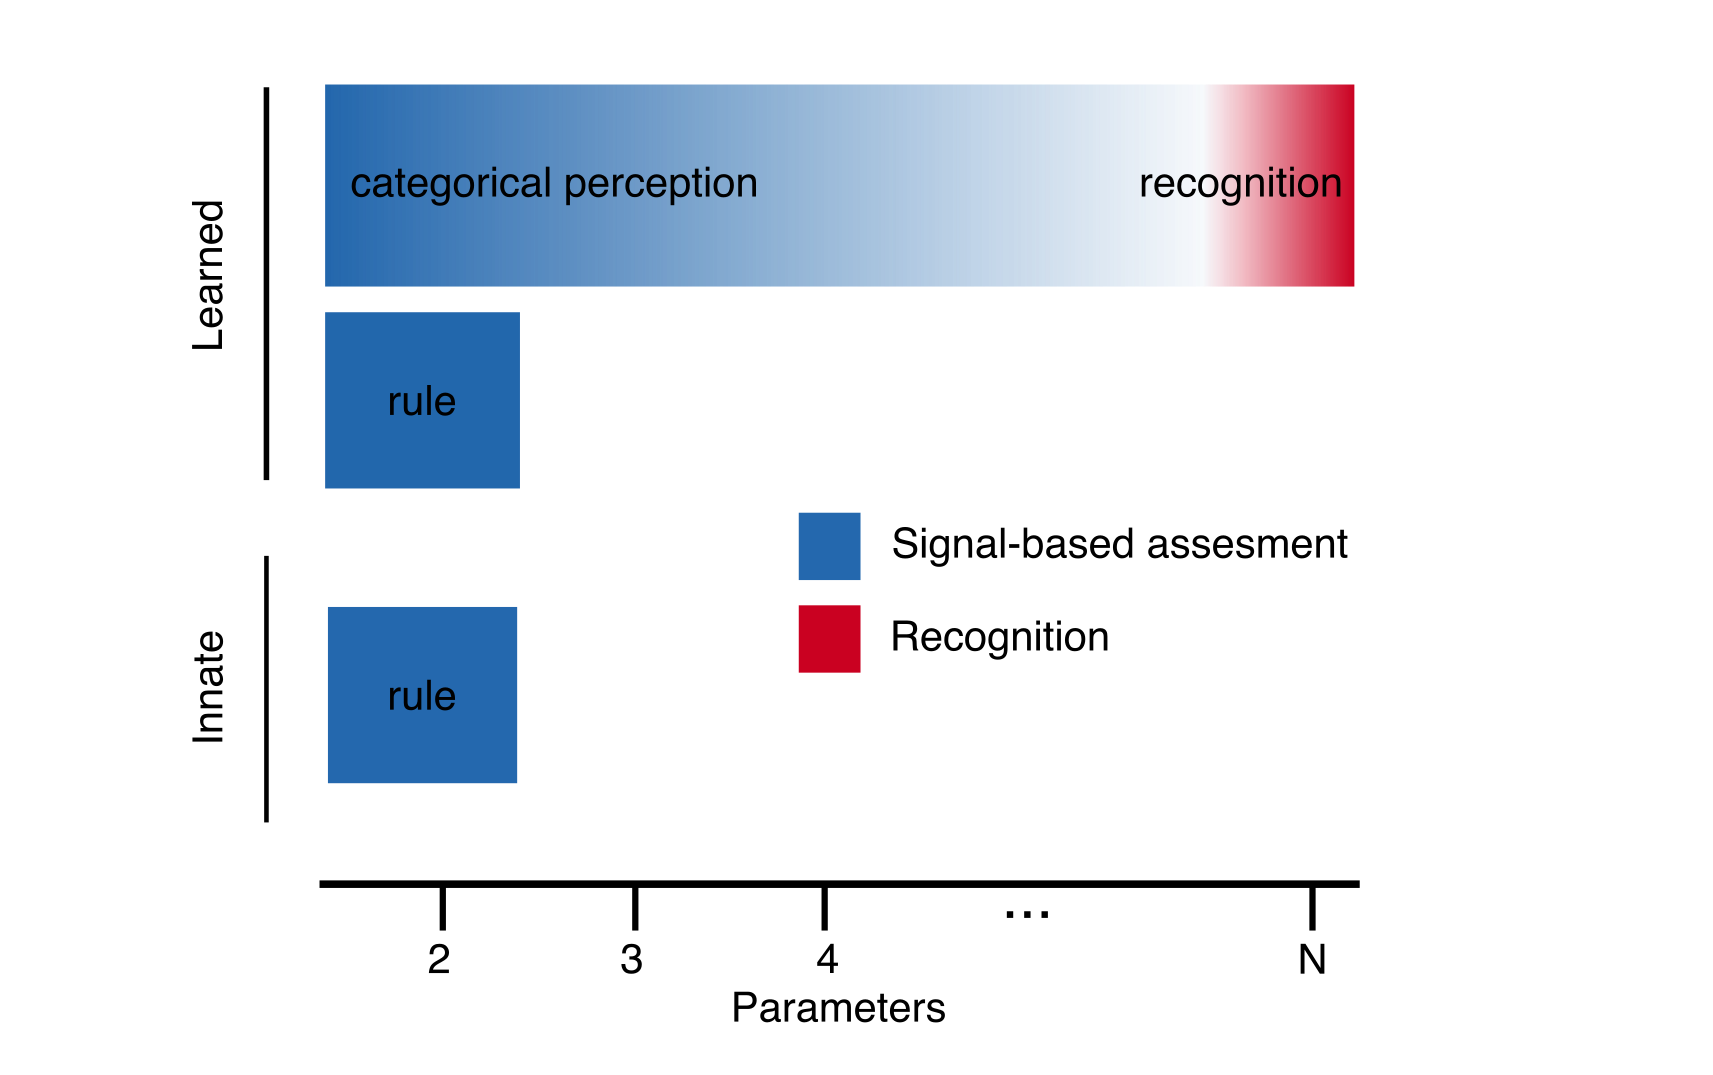
\includegraphics[width=6.85in]{figures/schematic_cropped.png}
\caption{\sffamily\small\textbf{Animals can use signals to infer the quality values of conspecifics.} They can do so using either a linear rule, which can be either learned or innate and which is determined by a slope and intercept, or categories, which can be coarse or fine. When there are as many categories as there are individuals in the group, categorical perception becomes individual recognition.}
\label{schematic}
\end{figure}

\begin{figure}
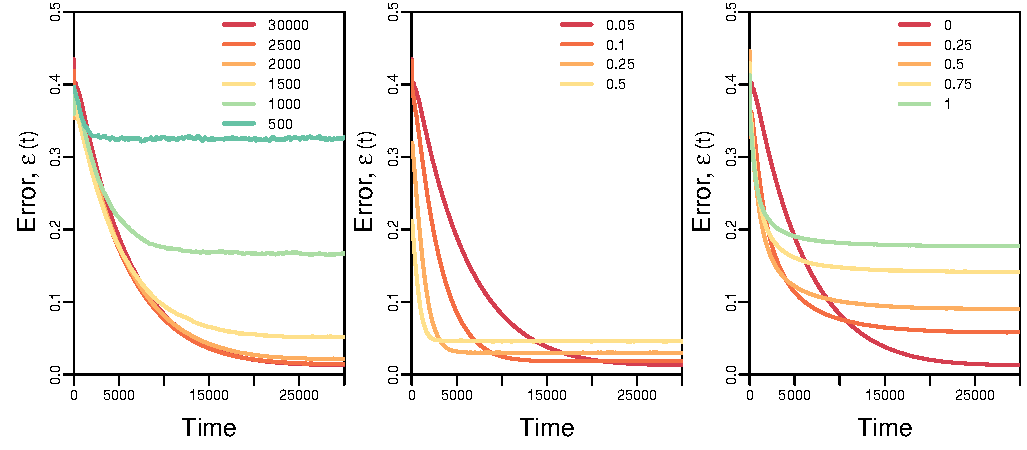
\includegraphics[width=6.85in]{figures/speed_accuracy_tradeoff.pdf}
\caption{\sffamily\small\textbf{As the animals learn, their errors decrease and eventually reach an equilibrium value.} Increasing the updating rate $r$ or category width $\delta$ helps the animals learn more quickly. When they have a long memory, this increases the equilibrium level of error, but when they have a short memory, it decreases the equilibrium level of error. In each panel, we show time $t$, in number of interactions, on the x-axis and the average error in an animal's assessment of its peers $\epsilon(t)$ on the y-axis. In each panel, light blue indicates animals using a learned rule, dark blue indicates animals using an innate rule, reddish colors indicates animals using recognition, and purple indicates animals using categorization. The points show the stopping time $\tau$ at which error stops decreasing (not shown for the innate rule because there is no learning). In A and B, the different reddish curves represent different updating rates. In C and D, the red and purple curves represent different category widths. In the left column, memory window $w=2500$ and in the right column, memory window $w=500$. Parameters: unless the parameter is being varied $\delta=0$, $N=25$, $r=0.05$, $\rho=0.99$.}
\label{tradeoff}
\end{figure}

\begin{figure}
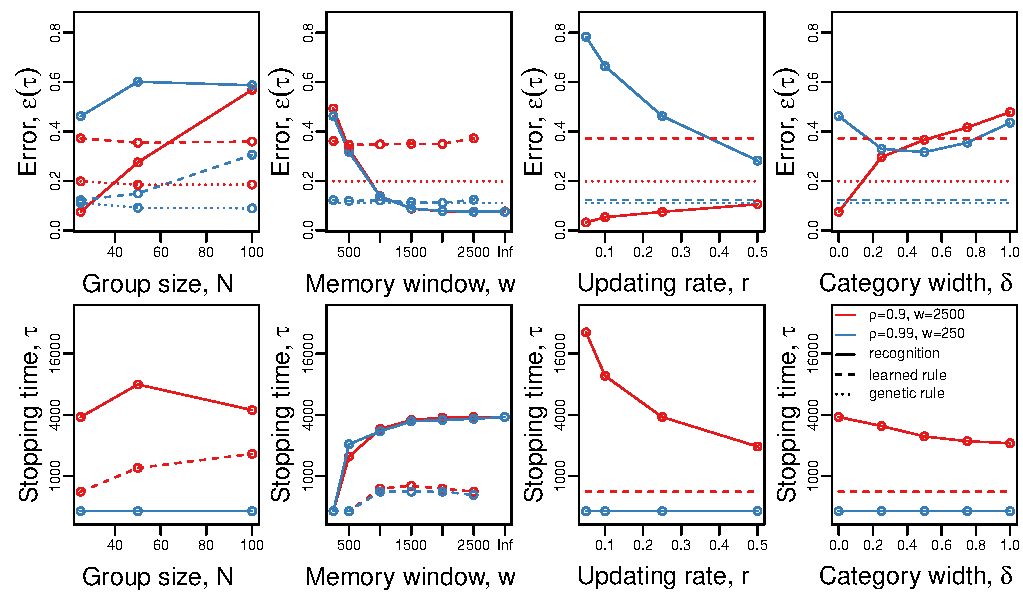
\includegraphics[width=6.85in]{figures/parameters_exploration.pdf}
\caption{\sffamily\small\textbf{Animals can learn about their peers with smaller errors when they have signals that are highly correlated with quality, live in small groups, and have long memory windows, and when errors are costly.} Here we show (A-D) stopping time $\tau$ and (E-H) average error $\epsilon(\tau)$, as a function of signal-quality correlation $\rho$, group size $N$, memory window $w$, and cost of errors $c$. Stopping time is on a logarithmic scale. In each panel, red curves show animals using recognition ($\delta=0$), purple curves show animals using categorization (with $\delta=0.25$), light blue curves show animals using a learned rule, and dark blue curves show animals using a innate rule. We do not show stopping time for animals using the innate rule because there is no learning involved.  The solid curves correspond to groups in which the signal-quality correlation $\rho=0.99$ and the dashed curves correspond to groups in which the signal-quality correlation $\rho=0.9$ (except in A and E, where we explicitly vary $\rho$). There are no dashed red curves because $\rho$ does not affect animals using recognition. The dark blue lines in G, and H do not have any points because these parameters, $w$ and $c$, do not affect the innate rule, so we show the value of $\epsilon(\tau)$ for animals using an innate rule as baseline to which we can compare the other strategies. `All' means that the animals can remember all of their interactions. We do not run the model of the learned rule with memory window equal to `All' because finding the regression of perceived quality values on observed signals values becomes unfeasible. Parameters: unless the parameter is being varied $c=1$, $N=25$, $r=0.5$, $w=2500$.}
\label{parameters}
\end{figure}

\begin{figure}
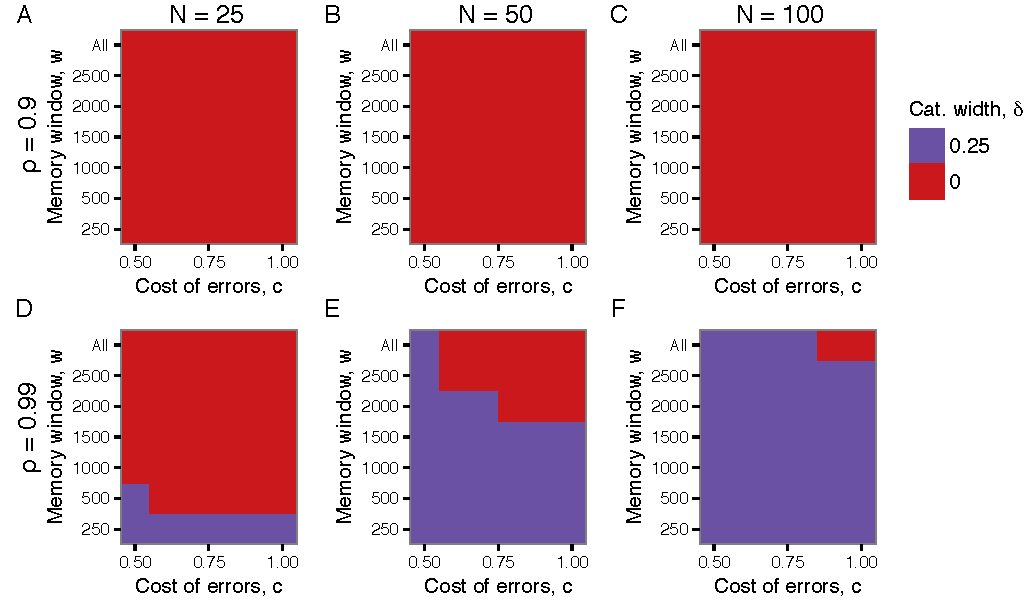
\includegraphics[width=6.85in]{figures/strategies_heat_maps.pdf}
\caption{\sffamily\small\textbf{Categorization is better than recognition when animals live in large groups, have short memories, when the signal-quality correlation is very high, and when errors are not very costly.} Here we show the optimal category width $\delta$, as a function of the cost of errors $c$ and memory window $w$. The optimal category width is the value of $\delta$ that minimizes the costs incurred from the combination of error and learning time. We concurrently find the value of $r$ that minimizes costs, as shown in Figure \ref{l}. When $\delta=0$ the animals are using individual recognition. `All' means that the animals can remember all of their interactions. In the first column, group size $N=25$, in the second column $N=50$, and in the third column $N=100$. Parameters: $\rho=0.99$. }
\label{opt_delta}
\end{figure}


\begin{figure}
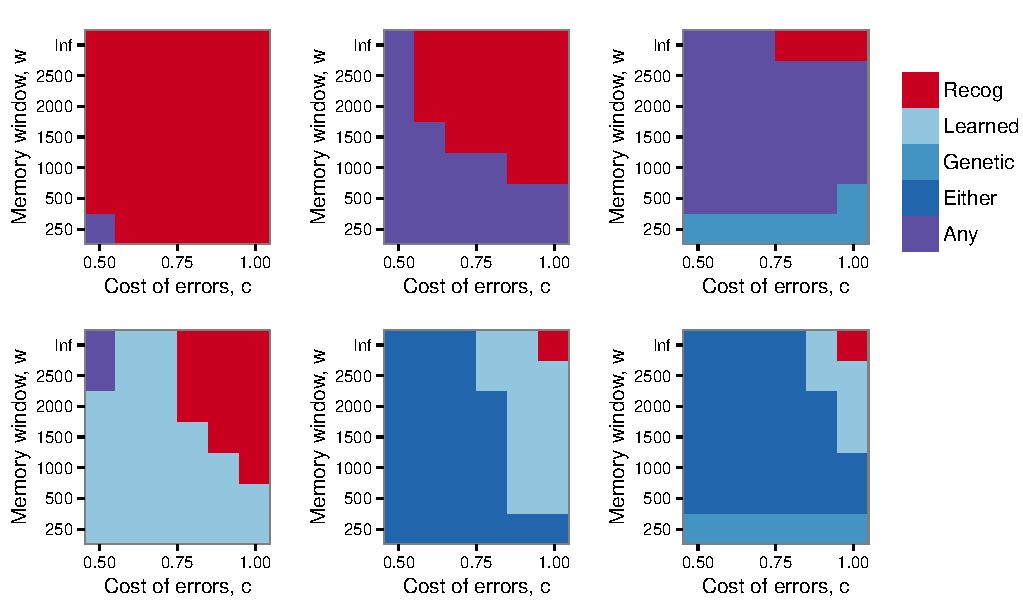
\includegraphics[width=6.85in]{figures/best_type_of_learning.pdf}
\caption{\sffamily\small\textbf{A rule is the best assessment strategy when animals live in large groups and have short memories, when the signal-quality correlation is very high, and when errors are not very costly.} Here we show which of the three assessment strategies---recognition, a learned rule, or a innate rule---is the least costly, as a function of the cost of errors $c$ and memory window $w$. Red indicates recognition is the least costly. Light blue indicates a learned rule is the best strategy. Intermediate blue indicates a innate rule is the best strategy. Dark blue indicates the two rules are essentially equally costly and less costly than recognition. Grey indicates the three strategies are all essentially equally costly. (Strategies are classified as equivalent if their costs are within $0.05$ of each other.) Using categorization ($\delta>0$) is never the best strategy (see also Figure \ref{opt_delta}). Animals using recognition are using the optimal stopping time $\tau$ and updating rate $r$ (Figures \ref{time} and \ref{l}, respectively). Animals using a learned rule are using the optimal stopping time $\tau$. `All' means that the animals can remember all of their interactions. We did not run the model of the learned rule with memory window equal to `All' because performing the required linear regressions is too computationally expensive. However, since memory window does not strongly affect the learned rule, we assumed that the performance animals using the learned rule with memory window `All' is equal to the performance of animals using the learned rule with memory window $2500$. In the first column $N=25$, in the middle column, $N=50$, and in the right column $N=100$. In the first row $\rho=0.9$ and in the second row $\rho=0.99$.}
\label{best}
\end{figure}

%
% \begin {table}[ht]
% \caption {Description of variables} \label{tab:vars} 
% \begin{tabular}{cl}

%  Variables & Description of variables \\
% \midrule 
% $a_{ij}(t)$ & animal $i$'s assessment of animal $j$ at time $t$ \\
% $C(t)$ & total cost of learning \\ 
% $c$ & cost of errors, whereas $1-c$ is the cost of spending time learning \\ 
% $\delta$ & category width (values near 0 = higher discriminatory ability, $\delta=0 \approx$ individual recognition)\\
% $e_{ij}(t)$ & error of animal $i$ about animal $j$ at time $t$\\
% $\epsilon(t)$ & average error of all animals in all groups at time $t$ \\
% $N$ & number of animals in group (small=25, medium=50, large=100)\\ 
% $\mathscr{O}_i(t)$ & set of animals about whom $i$ has an opinion at time $t$\\
% $q_j$ & quality of animal $j$ \\ 
% $\hat{q}_j$ & noisy information about the quality of animal $j$, $\hat{q}_j=q_j+\xi$ \\
% $r$ & updating rate (values near 0 = very fast updating rates)\\
% $\rho$ & sample correlation between quality and signal (high=0.9, almost perfect=0.99)\\
% $s_j$ & quality signal of animal $j$ \\ 
% $\sigma_\xi$ & standard deviation of noise in opinion updating during interaction, set to $0.1$ \\
% $\sigma_\text{q}$ & standard deviation of quality values, set to $0.5$ \\
% $T$ & total number of interactions, set to $30,000$ \\
% $\tau$ & stopping time \\
% $w$ & memory window (values near 0 = very short-term memory)\\
% $\xi$ & noise in the information animals get about each other's quality through interacting
% \end{tabular}
% \end {table}



\newpage
\begin {table}[ht]
\renewcommand*{\arraystretch}{1.4}
\caption {Description of variables} \label{tab:vars2} 
\begin{tabular}[t]{ |c|c|l| }
  \hline
  \multirow{6}{*}{\rotatebox[origin=c]{90}{\parbox{2cm}{\centering Interaction \\ parameters}}} 
  & $q_j$ 			& Quality of animal $j$ \\   
  & $\hat{q}_j$ 		& Noisy information about the quality of animal $j$, $\hat{q}_j=q_j+\xi$ \\ 
  & $s_j$ 			& Signal of animal $j$ \\ 
  & $\sigma_\xi$ 	& Standard deviation of noise in opinion updating during interaction, set to $0.1$ \\
  & $\sigma_\text{q}$ & Standard deviation of quality values, set to $0.5$ \\
  & $T$ 			& Total number of interactions, set to $30,000$ \\
  & $\xi$ 			& Noise in the information animals get about each other's quality through interacting \\
  \hline
  \multirow{5}{*}{\rotatebox[origin=c]{90}{\parbox{2cm}{\centering Assessment \\ parameters}}}
  & $c$ 				& Cost of errors, whereas $1-c$ is the cost of spending time learning \\ 
  & $\delta$ 	& Category width (ranges from $0$, meaning recognition, to $2$, meaning animals use $2$ categories)\\
 	& $N$ & Number of animals in group (we consider $N=25$, $50$, or $100$) \\
 	 & $r$ 		& Updating rate (we consider $r=0.05$, $0.1$, $0.25$, or $0.5$)\\
  & $\rho$ 		& Sample correlation between quality and signal (we consider $\rho=0.5$, $0.9$, or $0.99$) \\
  & $w$ 		& Memory window (we consider $w=250$, $500$, $1000$, $1500$, $2000$, $2500$, or `All', meaning every interaction)\\
  \hline
  \multirow{7}{*}{\rotatebox[origin=c]{90}{\parbox{2cm}{\centering Assessment \\ output}}} 
  & $a_{ij}(t)$ 		& Animal $i$'s assessment of animal $j$ at time $t$ \\
   & $C(t)$ 				& Total cost of learning \\ 
    & $e_{ij}(t)$ 		& Error of animal $i$ about animal $j$ at time $t$\\
  & $\epsilon(t)$ 		& Average error of all animals in all groups at time $t$ \\
  & $\mathscr{O}_i(t)$ 	& Set of animals about whom $i$ has an opinion at time $t$\\
  & $\tau$ 				& Stopping time \\

  \hline
\end{tabular}
\end {table}




%%%%%%%%%%%%%%%%%%%%%% FIGURES
%\clearpage
%\setcounter{figure}{0}

%\begin{figure}
%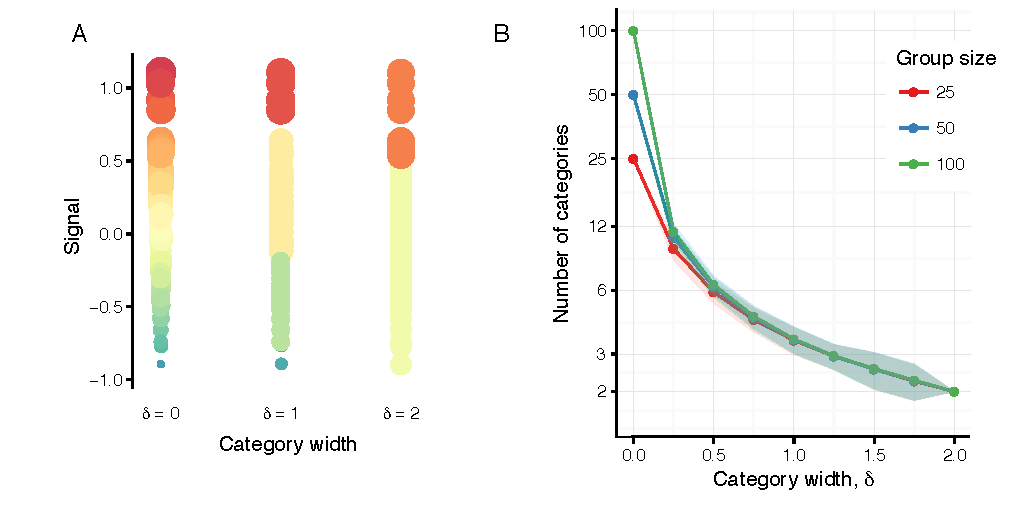
\includegraphics[width=6.85in]{figures/category_diagram.pdf}
%\caption{}
%\end{figure}

%\begin{figure}
%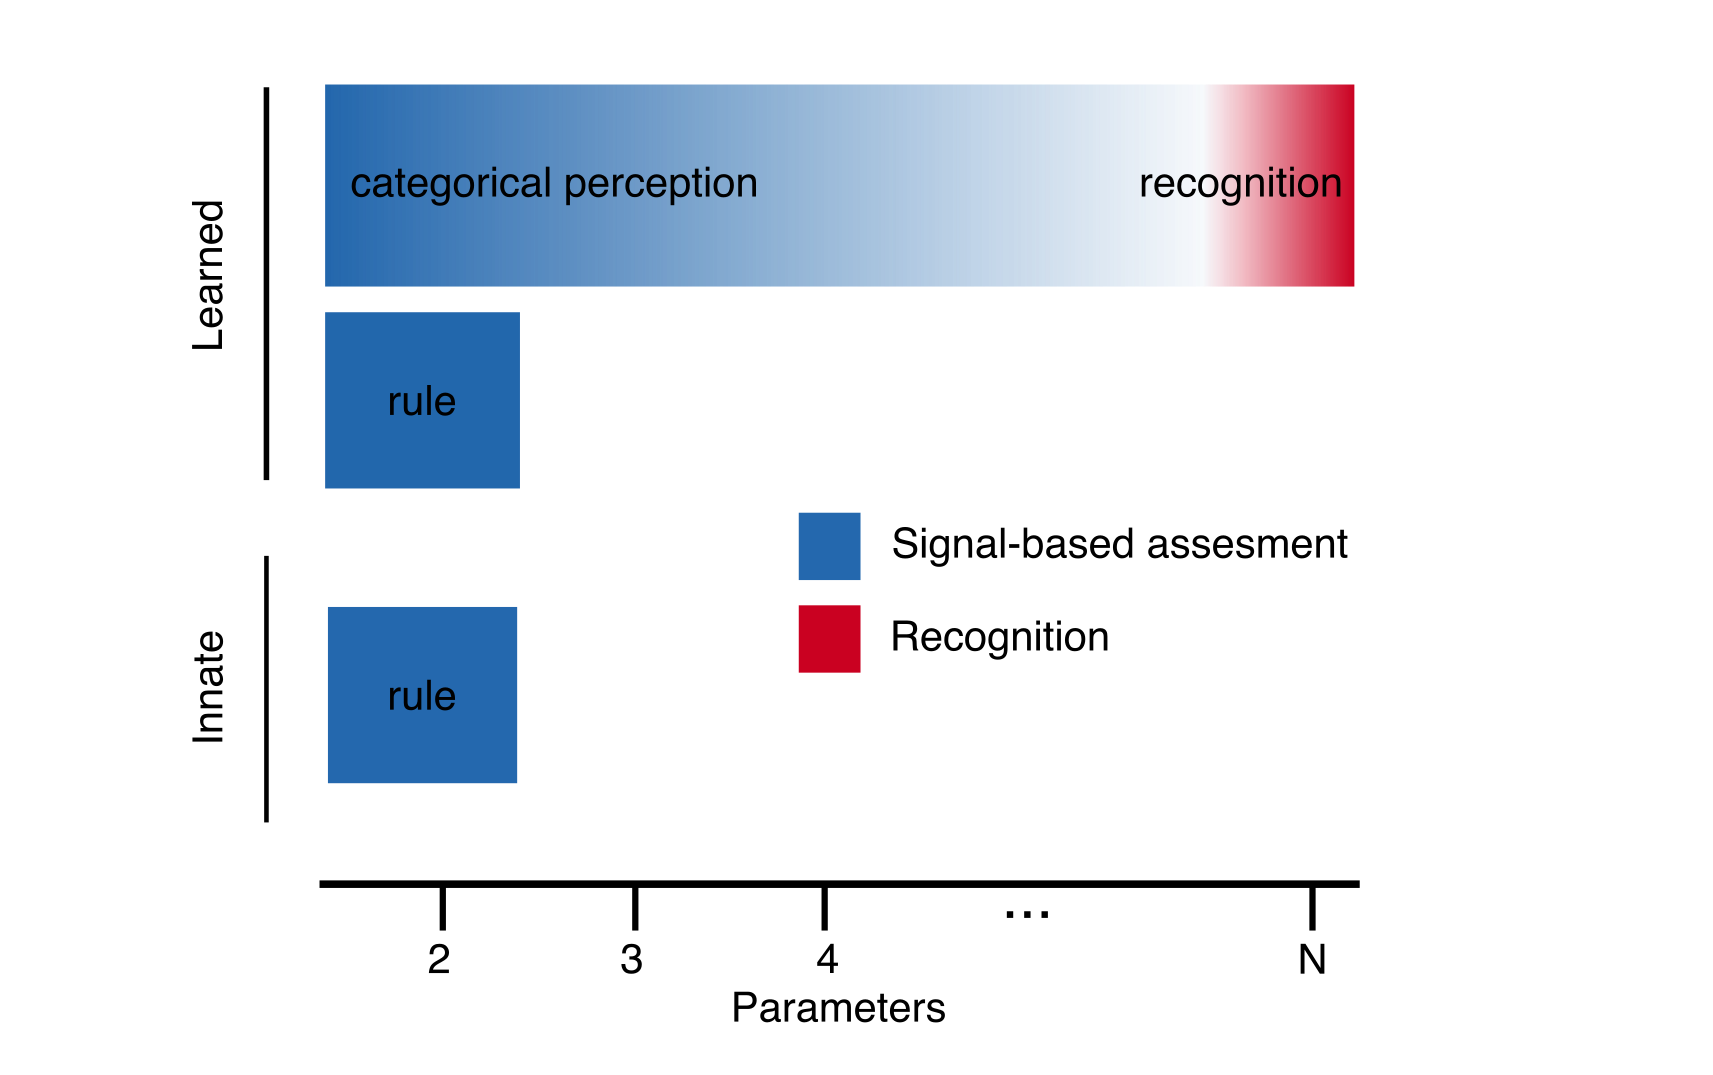
\includegraphics[width=6.85in]{figures/schematic_cropped.png}
%\caption{}
%\end{figure}

%\begin{figure}
%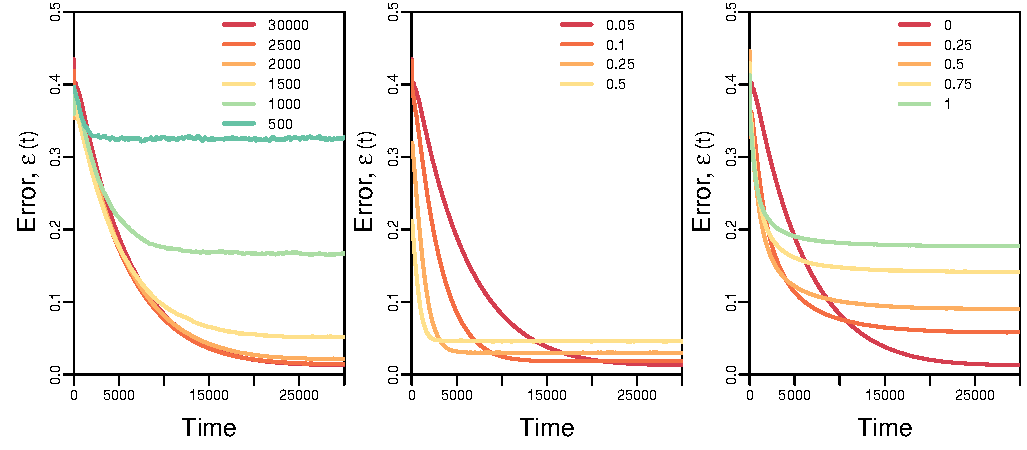
\includegraphics[width=6.85in]{figures/speed_accuracy_tradeoff.pdf}
%\caption{}
%\end{figure}

%\begin{figure}
%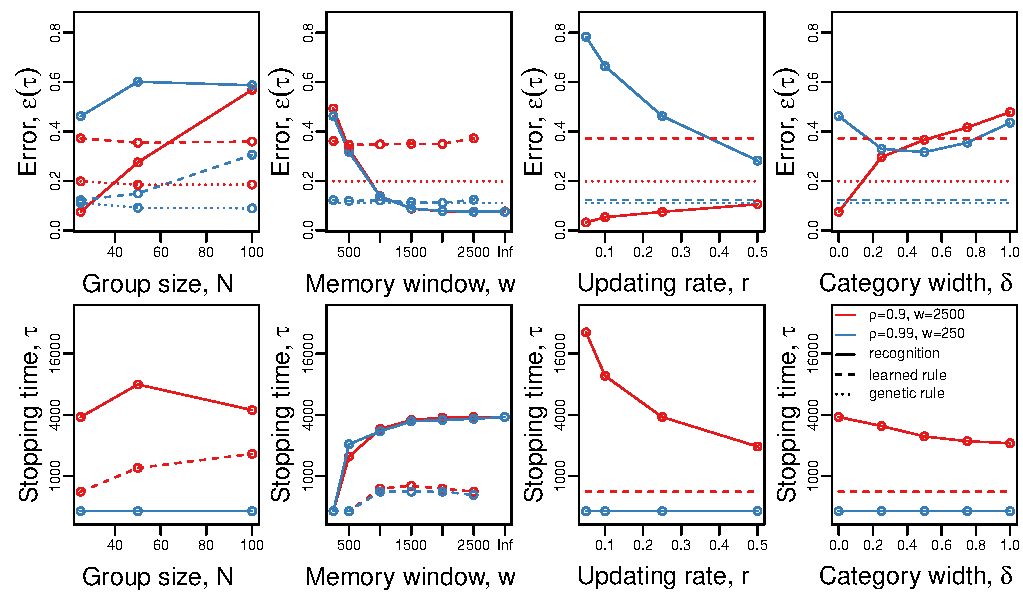
\includegraphics[width=6.85in]{figures/parameters_exploration.pdf}
%\caption{}
%\end{figure}


%\begin{figure}
%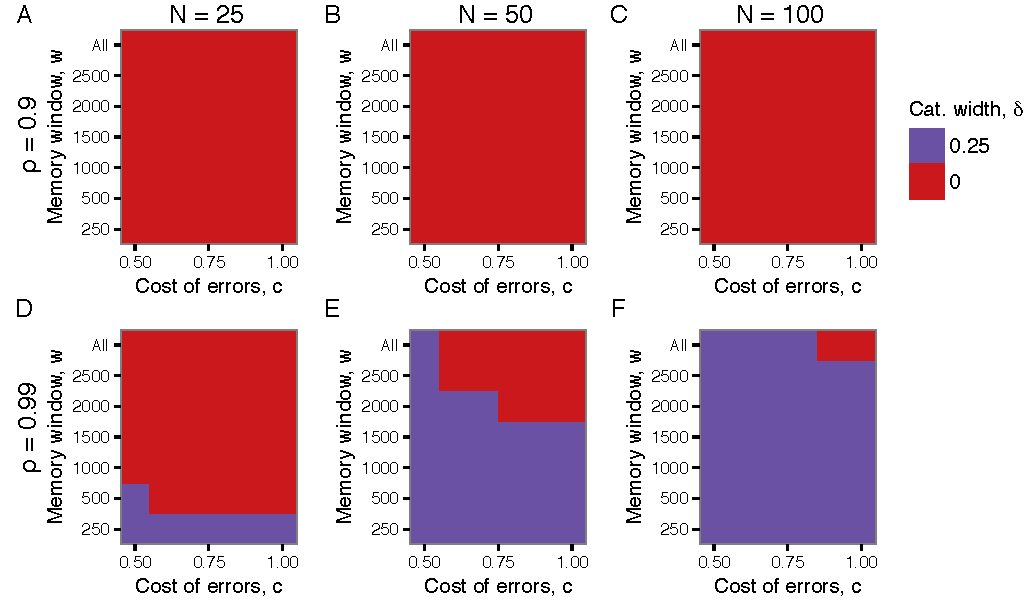
\includegraphics[width=6.85in]{figures/strategies_heat_maps.pdf}
%\caption{}
%\end{figure}


%\begin{figure}
%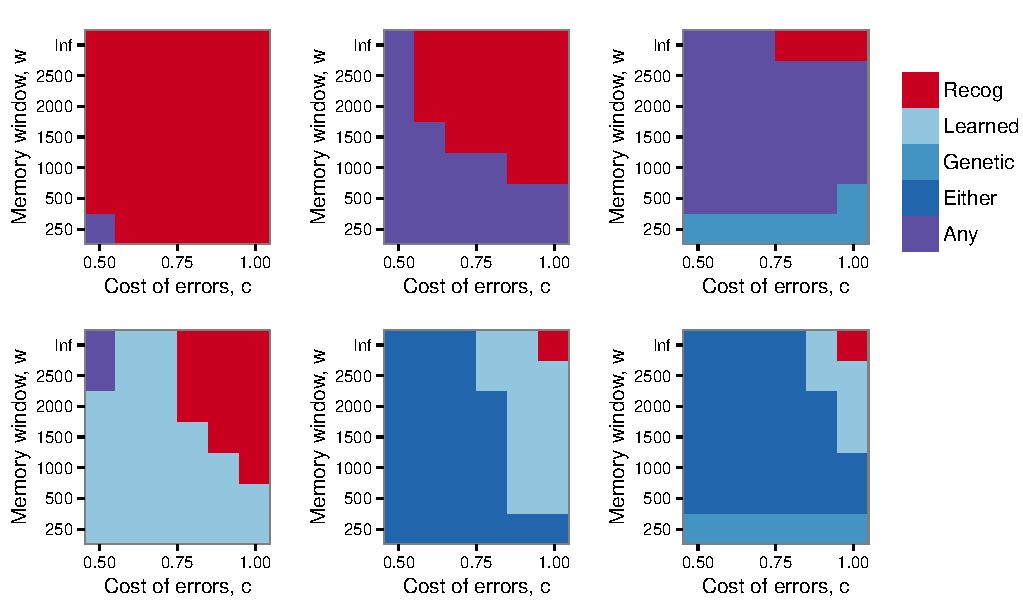
\includegraphics[width=6.85in]{figures/best_type_of_learning.pdf}
%\caption{}
%\end{figure}

\clearpage{}
\newpage{}
\renewcommand{\thesection}{}
\section{Supporting information}
\renewcommand{\thesection}{S}
\renewcommand{\thesubsection}{S\arabic{subsection}}
\renewcommand{\theequation}{S\arabic{equation}}
\renewcommand{\thetable}{S\arabic{table}}
\renewcommand{\thefigure}{S\arabic{figure}}
\setcounter{equation}{0}  
\setcounter{figure}{0}
\setcounter{table}{0}

\begin{figure}[ht]
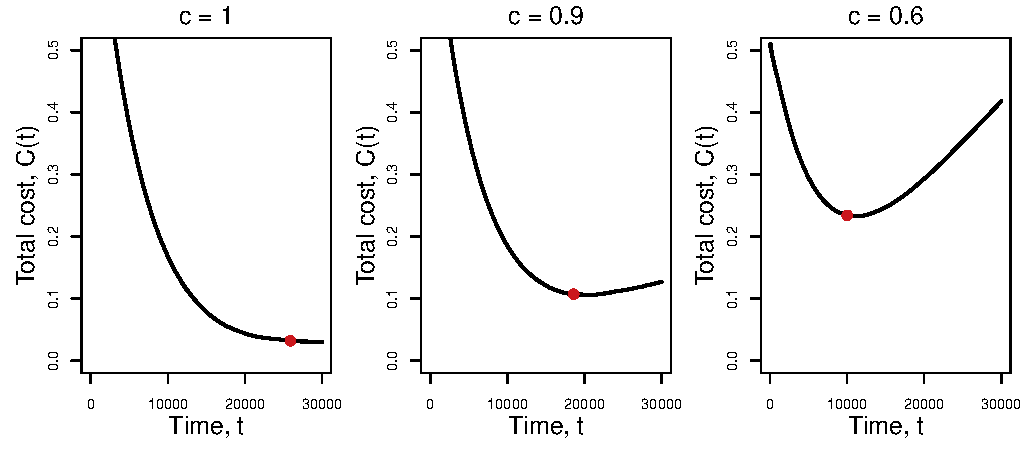
\includegraphics[width=6.85in]{figures/stopping_time.pdf}
\caption{\sffamily\small\textbf{As the cost of errors decreases and the cost of learning time increases, animals should stop learning earlier.} Here we show how we calculate stopping time $\tau$. In each panel, time $t$ in number of interactions  is on the x-axis and the total cost $C(t)$ is on the y-axis. In A, the cost of errors $c=1$: all that matters is error and the total cost $C(t)$ is equal to $2$ times the average error $\epsilon(t)$. In B, the cost of errors $c=0.9$ and in C, the cost of errors $c=0.6$: in each case, as time goes on, the animals incur costs from their interactions. In each panel, the stopping time $\tau$ is shown with the red point: this is the number of interactions at which the total cost $C$ stops decreasing and either plateaus or starts to increase. Parameters: $\delta=0$, $N=25$, $r=0.05$, $\rho=0.9$, $w=2500$.)
}
\label{tau}
\end{figure}


\begin{figure}[ht]
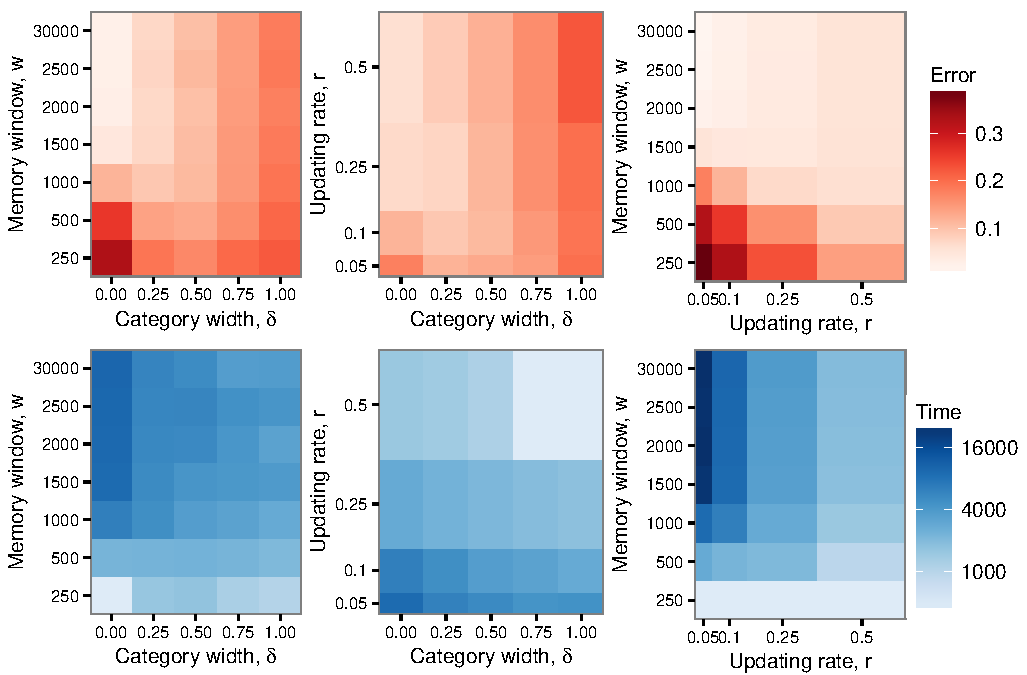
\includegraphics[width=6.85in]{figures/parameters_interactions_full.pdf}
\caption{\sffamily\small\textbf{Memory window, category width, and updating rate interact in their effects on how quickly and accurately animals using categorization can learn.}
Here we show stopping time $\tau$ (A-C) and average error $\epsilon(\tau)$ (D-F) for animals using categorization, as a function of two parameters. Stopping time is on a logarithmic scale. Increasing memory window increases stopping time (A and C) and decreases error (D and F). Increasing category width decreases stopping time (A and B). Intermediate category widths minimize error when memory and updating rate are low, but otherwise category width $\delta=0$ minimizes error (D and E). Increasing updating rate decreases stopping time (B and C). When memory window is low, increasing updating rate decreases error, but when memory window is high, increasing updating rate \emph{increases} error (F). Parameters: unless the parameter is being varied $\delta = 0$, $N=25$, $r=0.1$, $\rho=0.99$, $w=1000$. 
}
\label{interactions}
\end{figure}

\begin{figure}
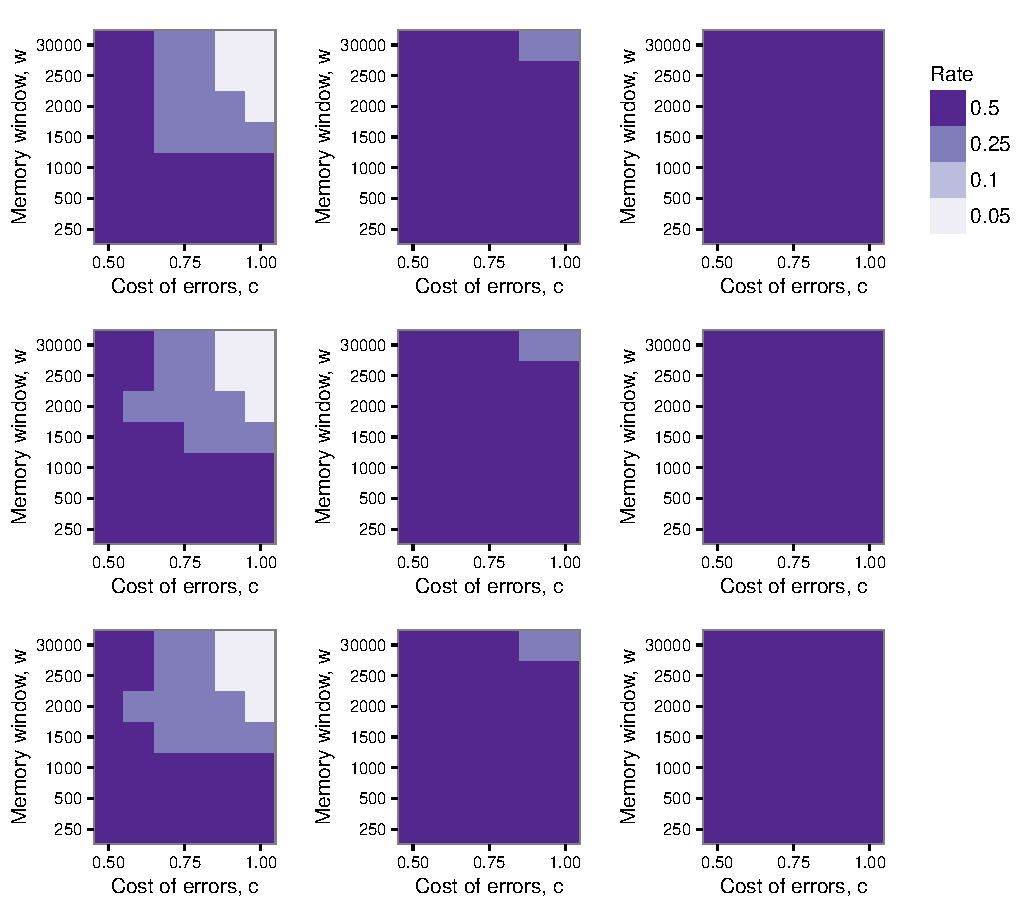
\includegraphics[width=6.85in]{figures/l_heat_maps.pdf}
\caption{\sffamily\small\textbf{} Here we show the optimal updating rate $r$ for animals using categorization, as a function of the cost of errors $c$ and memory window $w$. In the first column $N=25$, in the middle column $N=50$, and in the right column $N=100$. In the first row $\rho=0.5$, in the second row $\rho=0.9$, and in the third row $\rho=0.99$. The animals are also using the optimal stopping time $\tau$ and category width $\delta$, which are shown in Figures \ref{time} and \ref{opt_delta} respectively.}
\label{l}
\end{figure} 

\begin{figure}
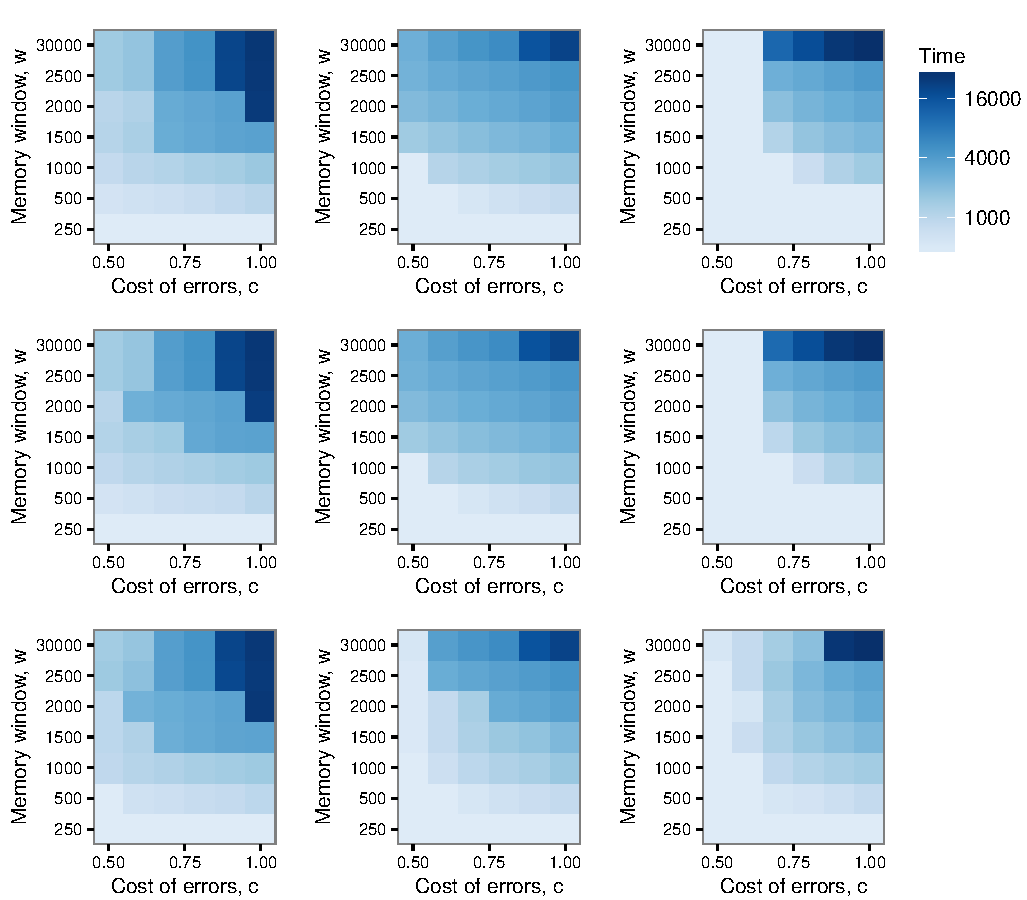
\includegraphics[width=6.85in]{figures/time_heat_maps.pdf}
\caption{\sffamily\small\textbf{} Here we show the optimal stopping time $\tau$ for animals using categorization, as a function of the cost of errors $c$ and memory window $w$. Stopping time is on a logarithmic scale. In the first column $N=25$, in the middle column $N=50$, and in the right column $N=100$. In the first row $\rho=0.5$, in the second row $\rho=0.9$ and in the third row $\rho=0.99$. The animals are also using the optimal category width $\delta$ and updating rate $r$, which are shown in Figures \ref{opt_delta} and \ref{l}.}
\label{time}
\end{figure}

%\begin{figure}
%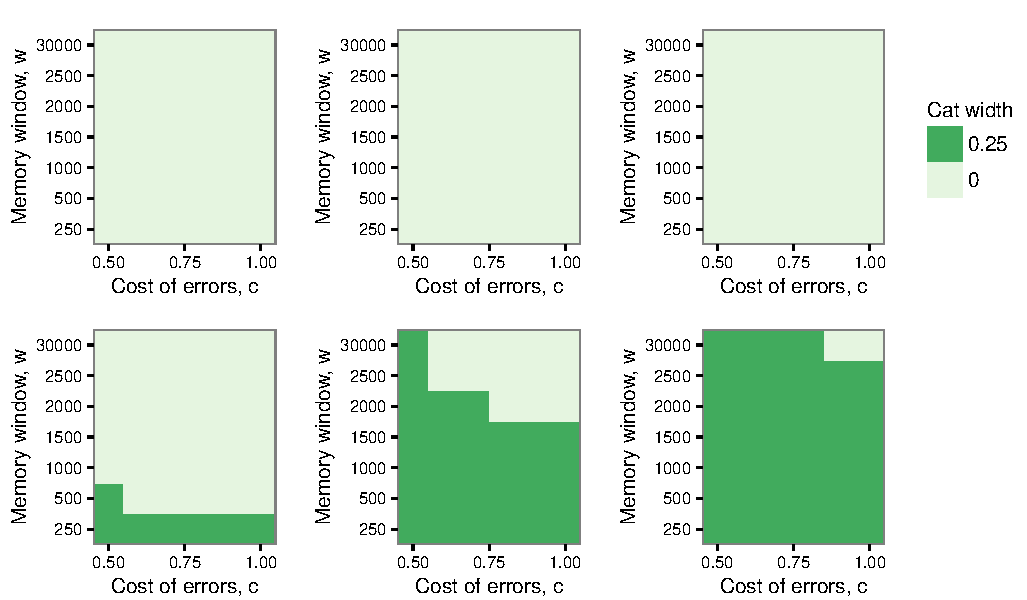
\includegraphics[width=6.85in]{figures/delta_heat_maps.pdf}
%\caption{\sffamily\small\textbf{Categorical recognition is better than individual recognition when animals live in large groups and have short memory windows and when the signal-quality correlation is very high.} Here we show how the optimal category width ($\delta$) animals using categorization depends on the cost of errors ($c$) and memory window ($w$). In the first column $N=25$, in the middle column $N=50$, and in the right column $N=100$. In the first row $\rho=0.5$, in the second row $\rho=0.9$, and in the third row $\rho=0.99$. The animals are also using the optimal stopping time ($\tau$) and updating rate ($r$), which are shown in Figures \ref{time} and \ref{l}.}
%\label{delta}
%\end{figure}

\begin{figure}
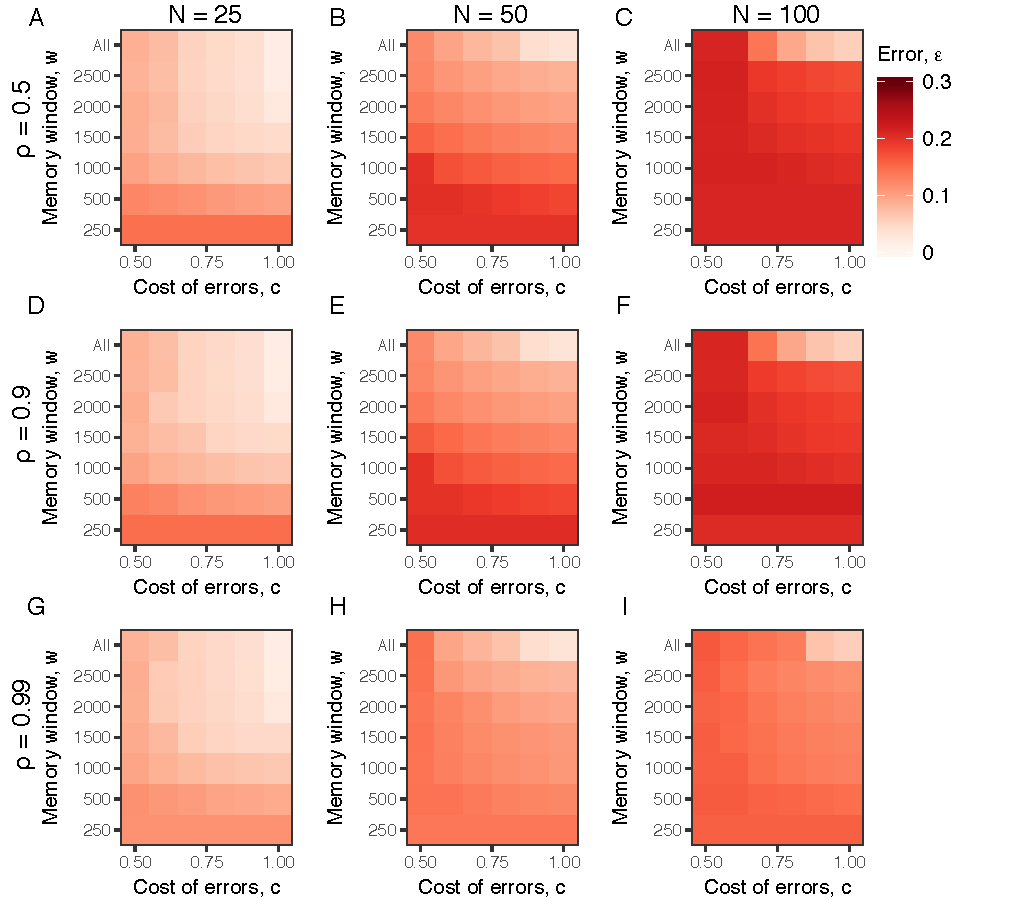
\includegraphics[width=6.85in]{figures/error_heat_maps.pdf}
\caption{\sffamily\small\textbf{} Here we show the average error $\epsilon(\tau)$ of animals using categorization, as a function of the cost of errors $c$ and memory window $w$. In the first column $N=25$, in the middle column $N=50$, and in the right column $N=100$. In the first  row $\rho=0.5$, in the second row $\rho=0.9$ and in the third row $\rho=0.99$. The animals are using optimal stopping time $\tau$, category width $\delta$, and updating rate $r$  as shown in Figures \ref{time}, \ref{opt_delta}, and \ref{l} respectively. }
\label{error}
\end{figure}


\begin{figure}
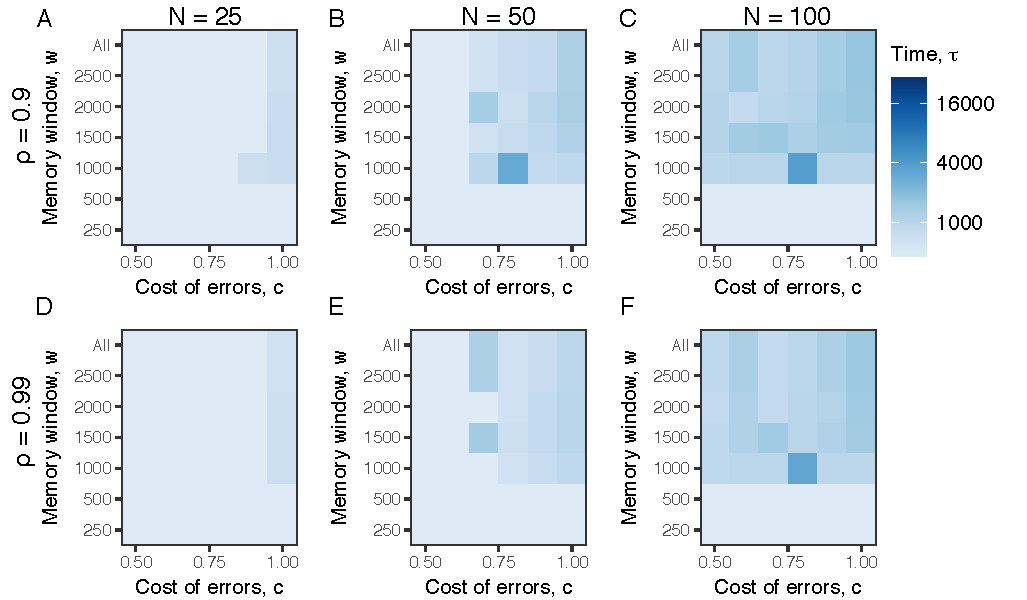
\includegraphics[width=6.85in]{figures/time_heat_maps_rule.pdf}
\caption{\sffamily\small\textbf{} Here we show how the optimal stopping time $\tau$ for animals using a learned rule depends on the cost of errors $c$ and memory window $w$. Stopping time is on a logarithmic scale. In the first column $N=25$, in the middle column $N=50$, and in the right column $N=100$. In the first row $\rho=0.9$ and in the second row $\rho=0.99$. }
\label{time_rule}
\end{figure}

\begin{figure}
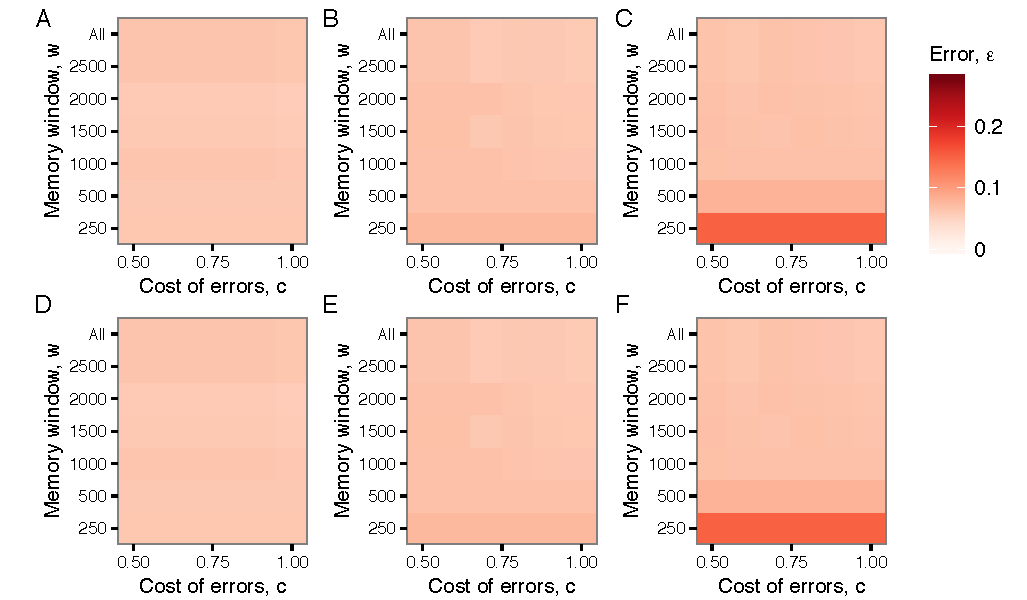
\includegraphics[width=6.85in]{figures/error_heat_maps_rule.pdf}
\caption{\sffamily\small\textbf{} Here we show how the average error $\epsilon(\tau)$ of animals using a learned rule with optimal stopping time $\tau$ (shown in Figure \ref{time_rule}) depends on the cost of errors $c$ and memory window $w$. In the first column $N=25$, in the middle column $N=50$, and in the right column $N=100$. In the first  row $\rho=0.9$ and in the second row $\rho=0.99$.}
\label{error_rule}
\end{figure}

%\begin{figure}
%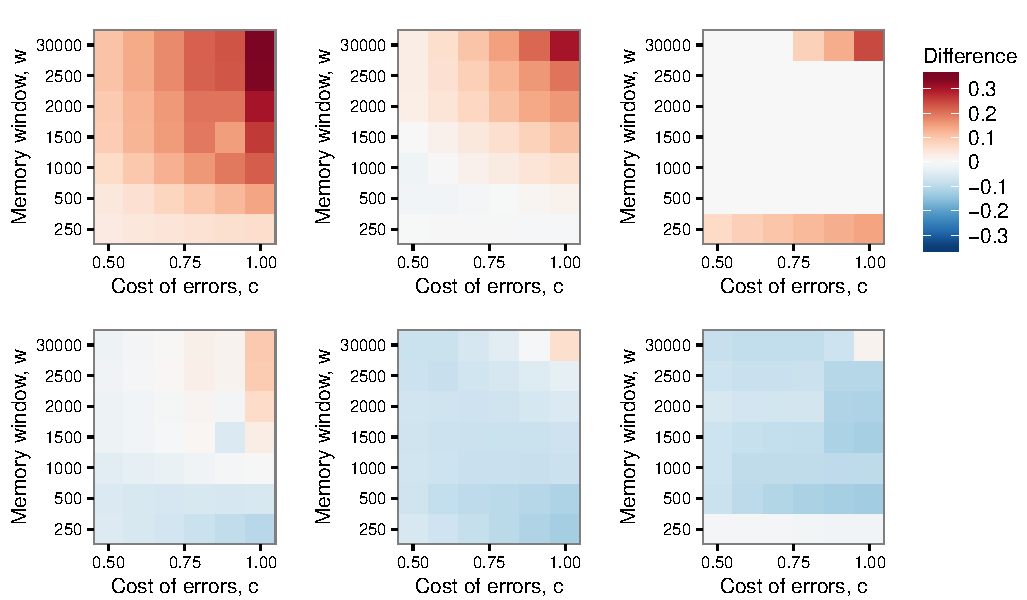
\includegraphics[width=6.85in]{figures/recog_vs_learned_rule.pdf}
%\caption{\sffamily\small\textbf{A learned rule is less costly than recognition (with optimized learning strategies) when animals live in large groups and have short memories and when the signal-quality correlation is high.} In each panel, we show the difference in overall costs between recognition and a learned rule as a function of the cost of errors $c$ and memory window $w$. Blue indicates a learned rule is less costly and red indicates recognition is less costly. The animals using recognition are using the optimal stopping time $\tau$, category width $\delta$, and updating rate $r$. In the first column $N=25$, in the middle column, $N=50$, and in the right column $N=100$. In the first row $\rho=0.9$ and in the second row $\rho=0.99$.}
%\label{comparison}
%\end{figure}

\begin{table}
\caption{\label{corr_examples} Examples of the correlation between a badge and a measure of fitness.}
\begin{tabular}{lllll}
Species & Badge & Measure of fitness & Correlation & Reference
\\\hline paper wasp & percent black on face & head width & $r^2=0.36$, for wasps  & Tibbetts \& Dale 2004
\\ & & & with $\geq 2$ black spots
\\ & ``badge brokenness" & dominance & $r^2=.105$ & Tibbetts \& Dale 2004
\\ \hline house sparrow & size of black bib & physical condition & $r=0.379$ & Veiga 1993
\\ \hline swamp sparrow & size of rusty cap & parental investment & $r^2=0.33$ & Olsen et al. 2010
\\ & size of black forehead & aggression & $r^2=0.41$ & Olsen et al. 2010
\end{tabular}
\end{table}

\end{document}
